\chapter{Iron in India From the Imperial Guptas to the Mighty Moghuls}\label{chapter5}

\lhead[\small\thepage\quad chapter V]{}

We have already seen that metallurgy of iron had gone through a long process of evolution and innovation over the centuries. It is the spirit of human endeavour which allowed man to innovate, improvise and master technology through experimentation. The technology of iron developed from simple wrought iron to steel, from tiny bits and small objects to colossal structures like victory pillars. In this chapter we propose to trace the developments and important features of iron technology between the period of the decline of the Gupta dynasty and the on-set of the mighty Moghuls. 

In Indian history as discussed earlier, $4^{\rm th}$-$5^{\rm th}$ centuries witnessed an era of prosperity, and overall growth in different fields. The Age of Imperial Guptas had earned the title of the Golden Age in Indian history. However, following the heydays of the Imperial Gupta rule, a decline gradually set in social, economic and political arena. With the disintegration of the central power, the country was divided into several small states being ruled by local rulers or the feudal lords of the Gupta Dynasty. One may wonder about the status of metal technology at this juncture of political turbulence. The provincial rulers had declared themselves independent. Feudalism dominated the socio-political system.  Internecine wars and feuds became the norm. In such a politically charged atmosphere, powerful army and weaponry assumed great importance. Weapons assumed paramount importance for those aspiring for gaining power. Naturally, demand for better, efficient and effective weapons, tools and implements grew manifolds. Under these circumstances the industries capable of providing military equipments, and weapons acquired greater significance. Victory pillars and commemorative monuments appear to have been erected by powers that be to assert their suzerainty. At the same time, the emerging powers asserted their presence with monumental structures, including religious architectures for the first time in India. The changing scenario promoted intensified activity in fields of art-architecture, masonry, building material etc. The rulers patronized talents many a times to boost up their egos and also to promote art-architecture, music, literature, science and technology as per their inclinations and interests. Treatises were composed on agriculture; industries like mining, and metallurgy; craft production. As a consequence, the knowledge system grew manifolds. Powerful trade guilds emerged. Industries and craft production attained greater heights. Under the trade guilds organized trade and commerce– prospered both over land and across the seas. The background for such growth was already prepared in the previous centuries as amply borne out by treatises like the Arthashastra of Kautilya. The Gupta period is a witness to affluence and prosperity in every sphere of life. The Mehrauli Iron Pillar datable to the Gupta period bears testimony to excellence achieved by the metallurgists in the field of iron technology.  Despite the decline in socio-political situation during the Post-Gupta period, the productive mechanism, trade and commerce continued to flourish. The robust economy with flourishing international trade and commerce was quite independent of state interventions. Alberuni had clearly stated of a disconnect between the political upheaval and economic activities. His oft quoted observation stating, ‘in India the farmers continued to till their fields while an army marched by’ is fully applicable in this context. With this brief background, we proceed to take a close look at the status of iron technology from the post- Gupta period to the Medieval Age. 

The flip side of such a state of affairs – foreign interactions, growing trade-commerce and prosperity of the land – is that it attracted many unwanted forces. Foreign invasions to acquire the famed riches of India became common phenomena. Frequent Muslim invasions not only looted the treasures housed in temples, their ruthless attitude attacked the very root on Indian socio-cultural system and weakened the very fabric of Indian society. They destroyed all that India of that age stood for– its philosophy, culture, education system which was build over the millennia. This fact is clearly borne out by the Arab and Persian accounts. The Arab and Persian scholars were shocked by the barbarity of the early Muslim invasions. The atrocities of these expeditions were the subject of intense dialogue among the contemporary scholarly world of the Middle East. This is clearly stated by Sheikh Bu Ali Sina who had refused to accompany Mahmud on his so-called jehad to India. Sina was an eminent Arab scientist philosopher. He strongly disapproved the fact that the invaders in the name of jehad  destroyed, among other things, Indian Science (Sarton 1931). Needless to state that Indian science received a serious jolt at the hands of such early Muslim invaders. Even Alberuni has written about how `Mahmud utterly ruined the prosperity of the country' and how {\it `Hindu sciences have retired far away'} (Sachau, reprint 1983). 

The libraries at ancient Universities of Taxla, Nalanda and Vikramshila were vandalized, totally burnt down. It is not surprising that texts on ancient sciences including those on iron metallurgy were lost in the process of burning down of libraries of the ancient universities. This badly harmed the scholarly tradition and nearly decimated the treasures of knowledge. King Bhoja of the famous Dhara Nagari (Dhar in Madhya Pradesh; 1010-1053 CE)) had composed a text on iron and steel technology. He also referred to three other texts composed on this subject prior to his own work. Such scientific literature seems to have been lost due to the turmoil and destruction caused by the plunders of early foreign invasions. What could survive the onslaught was only the practical knowledge prevalent among the practitioners of the technology. This has led to the assumption that these technologies (crafts?) were exclusively the prerogative of the so called lower classes or caste groups on Indian social system. The compositions by King Bhoj or other scholars have not been taken cognizance of as these works are lost and no longer available to us. Having examined the context of the era under review, we now proceed examine the status of iron technology at different stages during this period of Indian history.

\vspace{-.3cm}

\section*{Status of Iron From Imperial Guptas to\\ Early Medieval PERIOD}\label{chapter5-section-1}

\vspace{-.2cm}

During the Early Medieval Age there must have been pressure on the artisan class to produce iron objects in a large number, especially to assist in the agricultural and war sectors. Though the archaeology of early medieval times is not very well documented, the rich literary evidence of the period does provide valuable data on the socio-economic life. We have already discussed the masterpieces like the Delhi iron pillars that belong to this age ($4^{\rm th}$ –$6^{\rm th}$  century CE).

The accounts of an Egyptian-Greek merchant in his book {\it Periplus of Erythrian Sea} (Schoff 1912) testifies to the export of Indian iron to Abyssinia in the $1^{\rm st}$ half of the early centuries of the Common era. Periplus gives a detailed account of the voyages undertaken by its author and the ports he had visited. The most important harbour was Barygaza, a corrupted Greek form of Bhrigukachchha (modern Broach or Bharoch) on the mouth of the river Narmada. It was a busy port town where goods were brought in from distant parts of the subcontinent, like Kashmir and Hindukush mountains, so that they could be exported to foreign countries. Other port-towns mentioned in the text are Pratishthāna (Paithan), Tagars (Ter), Sopārā and Kalyāna (on Bombay coast). Several places on the Malabar Coast also find mention there. The ports of Muchiripattanam and Nilakanth mentioned there also yield old inscriptions saying that these places abound in ``ships sent there with cargoes from Arabia and by the Greeks". Indian ships almost regularly sailed to Arabian and African harbours. There is mention of a colony of Indian traders in the island of Socorta.

The articles of export from India were spices, perfumes, medicinal herbs, pigments, pearls, precious stones, iron and steel, copper, sandalwood, animal-skin, cotton cloth, silk yarn, muslin, indigo, ivory etc. Literary texts, both Brahmanical and Buddhist especially the Jatakas, refer to rich merchants. Both overland and sea trade prospered from $3^{\rm rd}$ –$2^{\rm nd}$ century BCE onwards. The luxury goods imported from India flooded the Roman cities. Pliny lamented that India drained the Roman Empire of its gold valued at fifty million {\it sesterces} and established a favourable trade balance in the foreign markets. There is no reason to doubt that the process must have intensified in the subsequent centuries. The technique of steel making was mastered as is evident from the textual data. As mentioned earlier, Varahmihir (c. 550 CE) gives an elaborate description of carburisation of sword blades: 

``Make a paste with the juice of the plant {\it Araka} ({\it Caleotropis gigantika}) mixed with gelatine from sheep's horn and the dung of pigeon or mouse. Apply it to the steel surface after rubbing it with sesame oil. Plunge the steel thus treated into fire and when it is red-hot sprinkle on it water or milk of mare (camel or goat), ghee or blood or fat or bile and continue the process for few hours. Then cool the sword blade, sharpen it on the lathe and then subject it to quenching and hardening treatment".\endnote{(Kharaglakshanam XLIX 23-26).}

There are also suggestions of similar kind at other places. They suggest plunging the red-hot sword into the solution of plantain ashes and whey and keeping it for twenty-four hours followed by grinding the blade on lathe. It could also be quenched by thrusting it directly into the trunk of plantain tree and allowing it to cool overnight. In view of metallurgists like Bhanu Prakash who tried to study and analyse such ancient practices, this would first convert the austenite into martensite and transform it into tempered martensite `due to reheating of the sharp edge of the blade by the flow of the heat from the thick back edge' (Prakash 2002).

Such descriptions suggest that the artisan communities of $5^{\rm th}$ –$6^{\rm th}$ century CE had developed quite complex processes of carburization and tempering. These processes must have already been in practice and were well established so as to find mention in important texts like the above one. Once perfected, the technique led to production of exclusive pieces that must have been in great demand in the contemporary world. 

During the earlier centuries of the period under discussion, there grew friendly and commercial interactions with the Arabs. In the Early Medieval times, Indian science and technology were at their peak. The early Arab writers of $9^{\rm th}$ –$10^{\rm th}$ centuries have written profusely about the astronomy, mathematics besides the agricultural practices, fertility of the soil, and several other techniques adopted by Indian cultivators.~They also refer to the metal and metal–working as a successful vocation of specialist craftsmen of this period. Abhidhānaratnamālā, a text of this period, makes a list of metals that includes copper, bell metal, iron and steel, lead, tin, silver and gold. Different parts of the country were famous for different metals. Agni Purana (CCXLV. 21) describes five centres that were famous for sword making. They are Khatīkhattara and Rishika (not identified so far), Surpāraka (Sopara), Vanga (Bengal) and Anga (Bhagalpur, Mungher districts of Bihar). Ibn Haukal\endnote{HEID History of India as told by its own Historians}, (HIED –1.37) mentions the city of Debal in Sind as a famous sword-making centre. Good quality swords were being produced also from iron or steel from Kurij in Kutch. 

These centres must have catered both to the local needs as well as to exports. The swords manufactured at several of the above mentioned places were very much in demand outside the country. In the following centuries frequent Mohammedan attacks and loots of riches became regular features. The political history of this period is too well known to warrant discussion here. The status of iron technology during this period may be examined in this perspective. The Geniza records of the eleventh and twelfth centuries bear testimony to the export of Deccan iron and steel to the Middle East, (Goitein 1966, 339). Fakhr-I-Mudabbir ($11^{\rm th}$ Century AD) thought that the Indian swords were the best. The Damascene sword or {\it Maujdarya} was considered exclusive, even by the Arab world. It is said that these swords could fetch the highest price in the world market. 

A fourteenth century AD work, {\it Sarangadhara Paddhati} (referred to by Joshi 1970: 82) by the alchemist Sarangadhara describes the technique of manufacturing swords. He mentions several important centres of sword making of his time.~Special mention may be made of Kahatikhattara, Rishika, Banga, Shurparaka, Videh, Anga (already mentioned in the Agni Purana, above), Madhyamgram, Bedidesha, Sahagram, Kalinjar. He has also given a detailed account of the quality of iron that was to be used for the manufacture of different types of swords. The colour of swords, according to him depended on the type of iron (ore?) that was used in their manufacture. It is unfortunate that the treatise is no longer available to us. 

Trade activity had intensified during this period ($10^{\rm th}$-$11^{\rm th}$ to $14^{\rm th}$-$15^{\rm th}$ centuries CE). Although an organised activity in trading sector had already started from the Buddhist times itself as evident from innumerable Jataka stories, the trade organizations– guilds or {\it shrenies} – had evolved as strong bodies with an identity of their own during the early medieval age. {\it Medhatithi} writes that both industrial and mercantile guilds functioned in his time. He defines (VIII, 41) the guild ({\it shrenis}) ``as consisting of people following common professions, such as tradesman, artisans, money lenders, coach driver, and so forth." (Ghoshal 1964: 405). They formed their own associations – {\it Sangha} who framed their own byelaws. In the $12^{\rm th}$ century CE, Hemachandra who\newpage lived in the court of king Kumarpala in Gujarat wrote about five distinct categories of organizations of big business enterprises:

\begin{enumerate}[(1)]
\item {\it Dravyaka}, an organization that lent money to invest in the trade.
\item {\it Vāstrika}, a business community dealing in cloths and fabric (?)
\item {\it Prāstārika}, an organization dealing in metals, like, gold, silver, copper, iron etc.
\item {\it Sānsthānika} – those engaged in animal trade
\item {\it Ārdhrakathinika} – those dealing in leather, lac, bamboo etc.
\end{enumerate}

These guilds wielded great power and sometimes even politically influenced the policies of the state; they carried out inland as well as international trade. Huge ocean going freights have been mentioned right from the times of Panini ($4^{\rm th}$ –$3^{\rm rd}$ century BCE). Colonies of Indian traders were established, outside the country also, as mentioned earlier. Thus commodities manufactured in different parts of the country were brought to the port towns and exported to different parts of the world, including the Arab world mentioned above, where the Indian swords were highly prized.

In the following centuries, the saliency of Indian iron is well testified by {\it Ras Ratna Samuchchaya} (RRS), a $11^{\rm th}$ -$12^{\rm th}$ century text on alchemy. It is not difficult to assume that a well-developed scientific basis must have evolved giving authentic material like the ones documented in RRS in great detail. A very fine classification of different types of iron has been attempted in the text showing a deep understanding of behaviour of iron in the smelting-refining process. Three basic types of iron with different sub-types (according to their properties and nature) have been categorised in {\it RRS}, which may be systematized as under:
\newpage
{\setcounter{table}{0}
\renewcommand{\thetable}{V.\arabic{table}}
{\fontsize{8}{10}\selectfont
\begin{longtable}{|p{.8cm}|p{1.3cm}|p{5.6cm}|}
\caption{Classification of Iron as in RRS}\label{table V.1}\\
\hline
{\it Kant Loha} & {\it Bhramaka}\par  {\it Chumbaka}\par {\it Drawaka}\par {\it Romaka} & Very soft magnetic iron\par Mildely magnetic\par One which can pull\par Paramount magnet, having strong magnetic field. It could be {\it ekmukha} (single direction) or {\it sarva mukha}  (multi directional)\\
\hline
{\it Tikshna Loha} & {\it Khara} \par {\it Sara}\par {\it Hrnnala}\par {\it Taravaratta} \par {\it Vajra }\par {\it Kalayasa} & 
With good cutting edge, may break easily \par Soft; fibrous fracture \par Hard, tough-fibrous structure, Good cutting edge \par Good hardening tempering property; \par Bluish in hue and hard cutting edge \par Develops hard cutting edge after tempering\\
\hline
{\it Munda Loha} & {\it Mridu} & Soft brittle, may be grey cast iron, has low melting point\\
& {\it Kunth} \par {\it Kadara} & Mottled grey iron \par White cast iron\\
\hline
\end{longtable}
}}
Such a comprehensive classification of different types of iron could have evolved only after a long period of intensive research. This is reflected best in the massive pillars and beams that we come across during early the medieval periods in several parts of the country.

Prakash (1991) and Biswas (2001) have tried to translate the terms of {\it RRS} into modern terminology:

{\it Kanta loha} is soft wrought iron with five sub-varieties of different magnetic properties. Prakash thinks that the name {\it munda loha} (a major variety) probably originated from {\it mundia}, one of the metalsmith tribes in the district of Bastar whose traditional iron making process has been scientifically observed and recorded by Prakash and Igaki. (1984). {\it Munda loha} had three sub varieties: {\it mridu}, soft which is {\it drutadrava} ‘melting or softening quickly’ and could have had a low melting point grey cast iron; {\it kuntha}, which expanded with great difficulty on hammering, could be a mottled grey iron; and {\it kadara} sub-variety which ‘breaks on hammering’ could be white cast iron. The indigenous metal smiths produced the last two brittle varieties unintentionally, when the temperature of the furnace became high and the amount of charcoal used was large, it resulted in high carbon iron. They preferred the first variety {\it medu}, which had smooth surface and did not contain fissures. This variety was adjudged to be ‘ the best of the three.’

{\it Tiksna-loha} or carbon steel had six sub-varieties. These appreciably hard sub-varieties were carburised iron that could be hypo-eutectoid (less than 0.83 percent carbon) or hyper-eutectoid (more than 0.83 percent carbon) steel. {\it Pogaras} mentioned in the text ({\it RRS}, 5.77-83) meant hair like lines, which could be white cementite streaks, coarse enough to be seen by the naked eyes.

\footnotesize{“The {\it khara} sub-variety of {\it tikshna–loha} is free from {\it pogaras} (or it is too fine to be seen), breaks on bending and has ‘mercury-like shining fractured surface’. The {\it sara} sub –variety appears to be fibrous. The other four varieties were probably the products of hot forging and quenching. {\it Hrnnala} looked whitish black and contained {\it pogaras}; this was {\it `chedane atiparusam'}, i.e. one that was very difficult to pierce. {\it Vajra} looked bluish black and was ‘full of hard {\it pogaras} and overspread by dense thin linings.’ {\it Tārāvatta} developed good cutting edge. {\it Kālāyasa} was described as ‘bluish black in colour, dense, smooth, heavy and bright in appearance, whose sharpened edges do not get spoiled even by hammering.’ This description is close enough to that of the Damascened steel swords ‘of a dull blue colour marked with ten millions of meandering lines’ which are compressed and elongated cementite grains or streaks in pearlite-graphite-martensite matrix”} maintains Biswas (op.cit. 121.)

One may easily get an insight into the supremacy of the metallurgical skills on the basis of the fine classification of the different types of steel that the workers of the age were capable of turning out. Such steel was occasionally commissioned by the rulers who wished to immortalize their victories and achievements. This attitude resulted into construction of massive monumental structures of iron, some of the important examples of the above are: the victory pillar at Dhar and the large beams at Konark. Some of these monumental structures are being mentioned below.	

\vspace{-.3cm}

\subsection*{The Monumental Structures}\label{chapter5-subsection-1}

\vspace{-.2cm}

Large sized structures of iron like pillars, beams etc. used in monumental buildings are found in several parts of the country. The frequently mentioned examples are the Delhi iron pillar of $5^{\rm th}$ century CE weighing over 6096 kg- nearly 7 tons (also mentioned in the previous chapter ), and the iron beams at Konark temple datable to $9^{\rm th}$-$10^{\rm th}$ century CE, which lie in several pieces in the temple complex. Its longest piece is 11,000 mm in length and 175x 197 mm in cross section and weighs approximately 3000 kg.

\noindent \textbf{\large The Delhi Iron Pillar}

The Delhi iron pillar (Fig.~28) has been an enigma to the historians and metallurgists of the world alike. This pillar, also known as Mehrauli iron pillar has withstood corrosion for nearly 1600 years. It is a wrought iron pillar. The iron was obtained by solid-state reduction, a technique that has been in vogue in India through the ages. The ancient Indian smiths had a thorough knowledge of the importance of carbon alloying and probably also that of hardening and tempering. Such technical skills must have been acquired over a long period before the craftsmen could venture to take up such a challenging job of manufacturing an iron pillar, which was 416 mm in diameter and 7,375 mm in height. This iron pillar is said to be made at Vishnupada (probably Mathura) and brought to the present site at Delhi around A.D. 1050 by King Anangapada II.

\newpage

Hadfield (1925) had examined this pillar and analysed the iron. He proposed that the purity of the iron was the prime factor for the resistance to corrosion. However, it was discovered from later studies that the wrought iron of the Delhi pillar is heterogeneous (Ghose 1963; Bardgett and Stanners 1963) and hence the pure metal theory of Hadfield may not be correct. Ghose (1963) attributes the corrosion resistance quality to low sulphur and impurity content, and excellent forge welding technique. He has mainly attributed the corrosion resistance of the pillar to the absence of manganese/sulphur and presence of high phosphorus in the iron of the pillar.

For manufacturing the Delhi Iron Pillar at least 8,000 kg of iron must have been used and as per published records the largest iron-making furnace of Nagpur (Fig.~49, pre-industrial iron working dated to $19^{\rm th}$ century) could produce about 40 kg of iron per heat. Thus, at least 200 furnaces would have to be operated simultaneously or the same furnace would have been used repeatedly to produce this amount of iron of consistent quality. The iron produced from each heat was hot­ forged to squeeze out the slag and then shaped into rods of 15 to 20 mm cross-section. In the absence of any documentation of the type of forging anvil, hammer and the hot metal handling tools used in the manufacture of such large objects, so far are left to our speculation (Prakash and Tripathi 1986). R. Balasubramania has extensively studied the metallurgy and logistics of the Delhi Iron Pillar in recent years from various angles. He has discussed these points in greater detail in a separate volume in this series (Balasubramaniam 2008).

\begin{figure}[H]
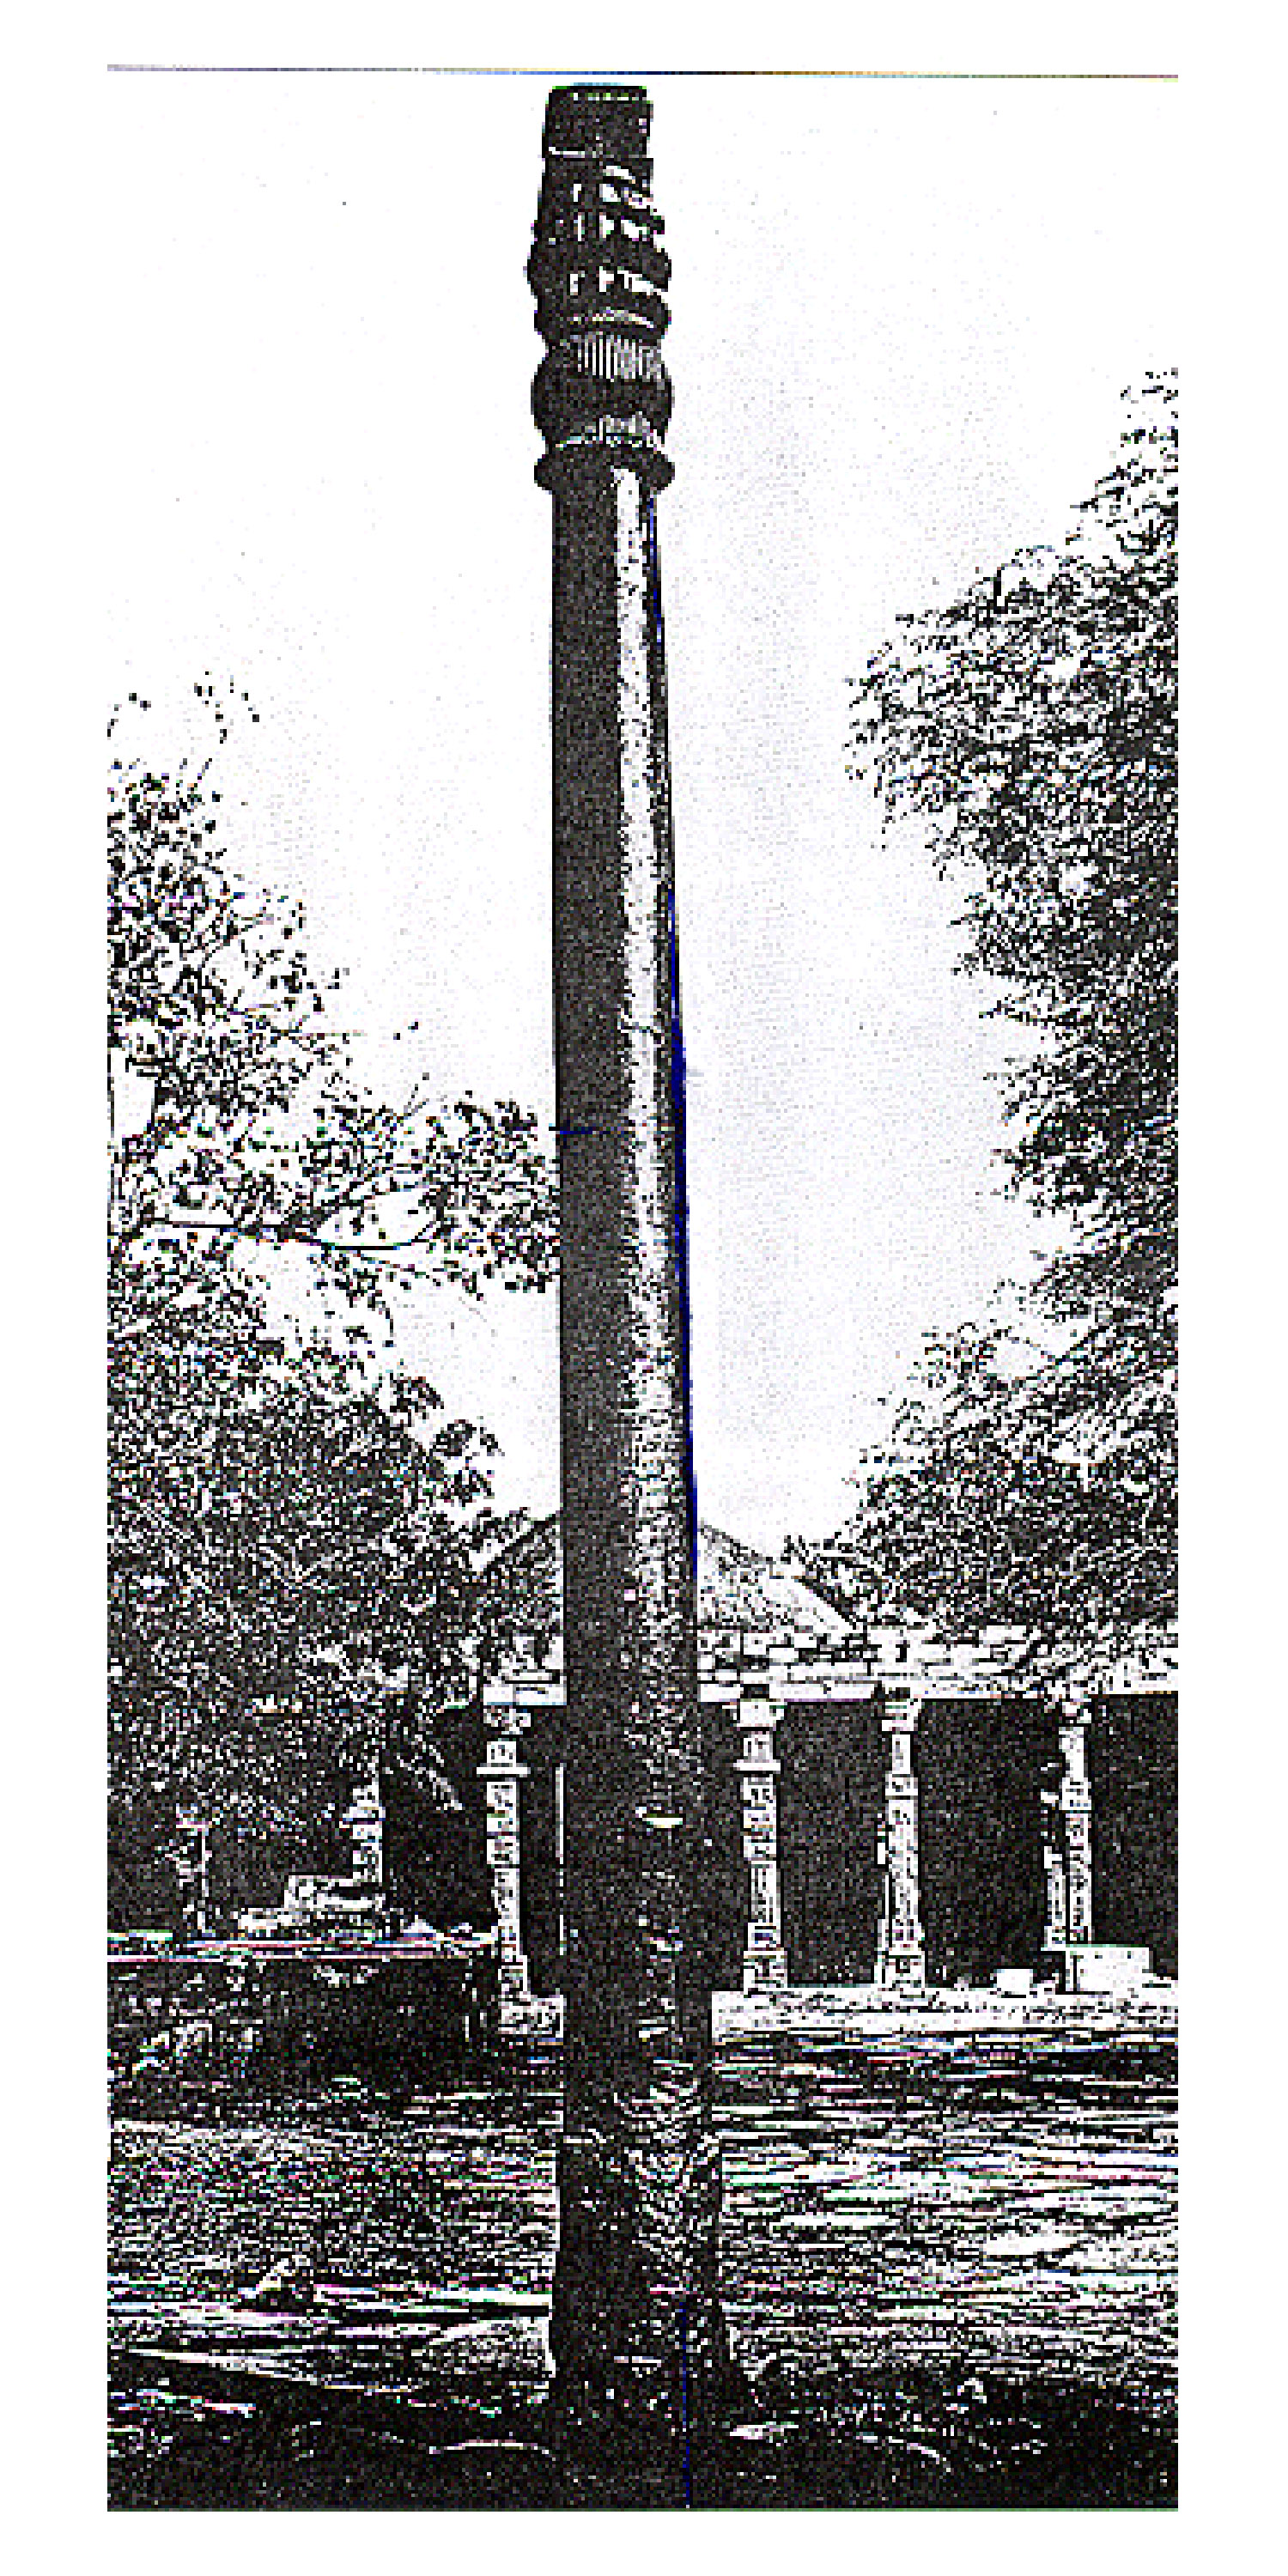
\includegraphics[scale=.5]{images/chapter-5/Fig28A.jpg}
\end{figure}
\begin{figure}[H]
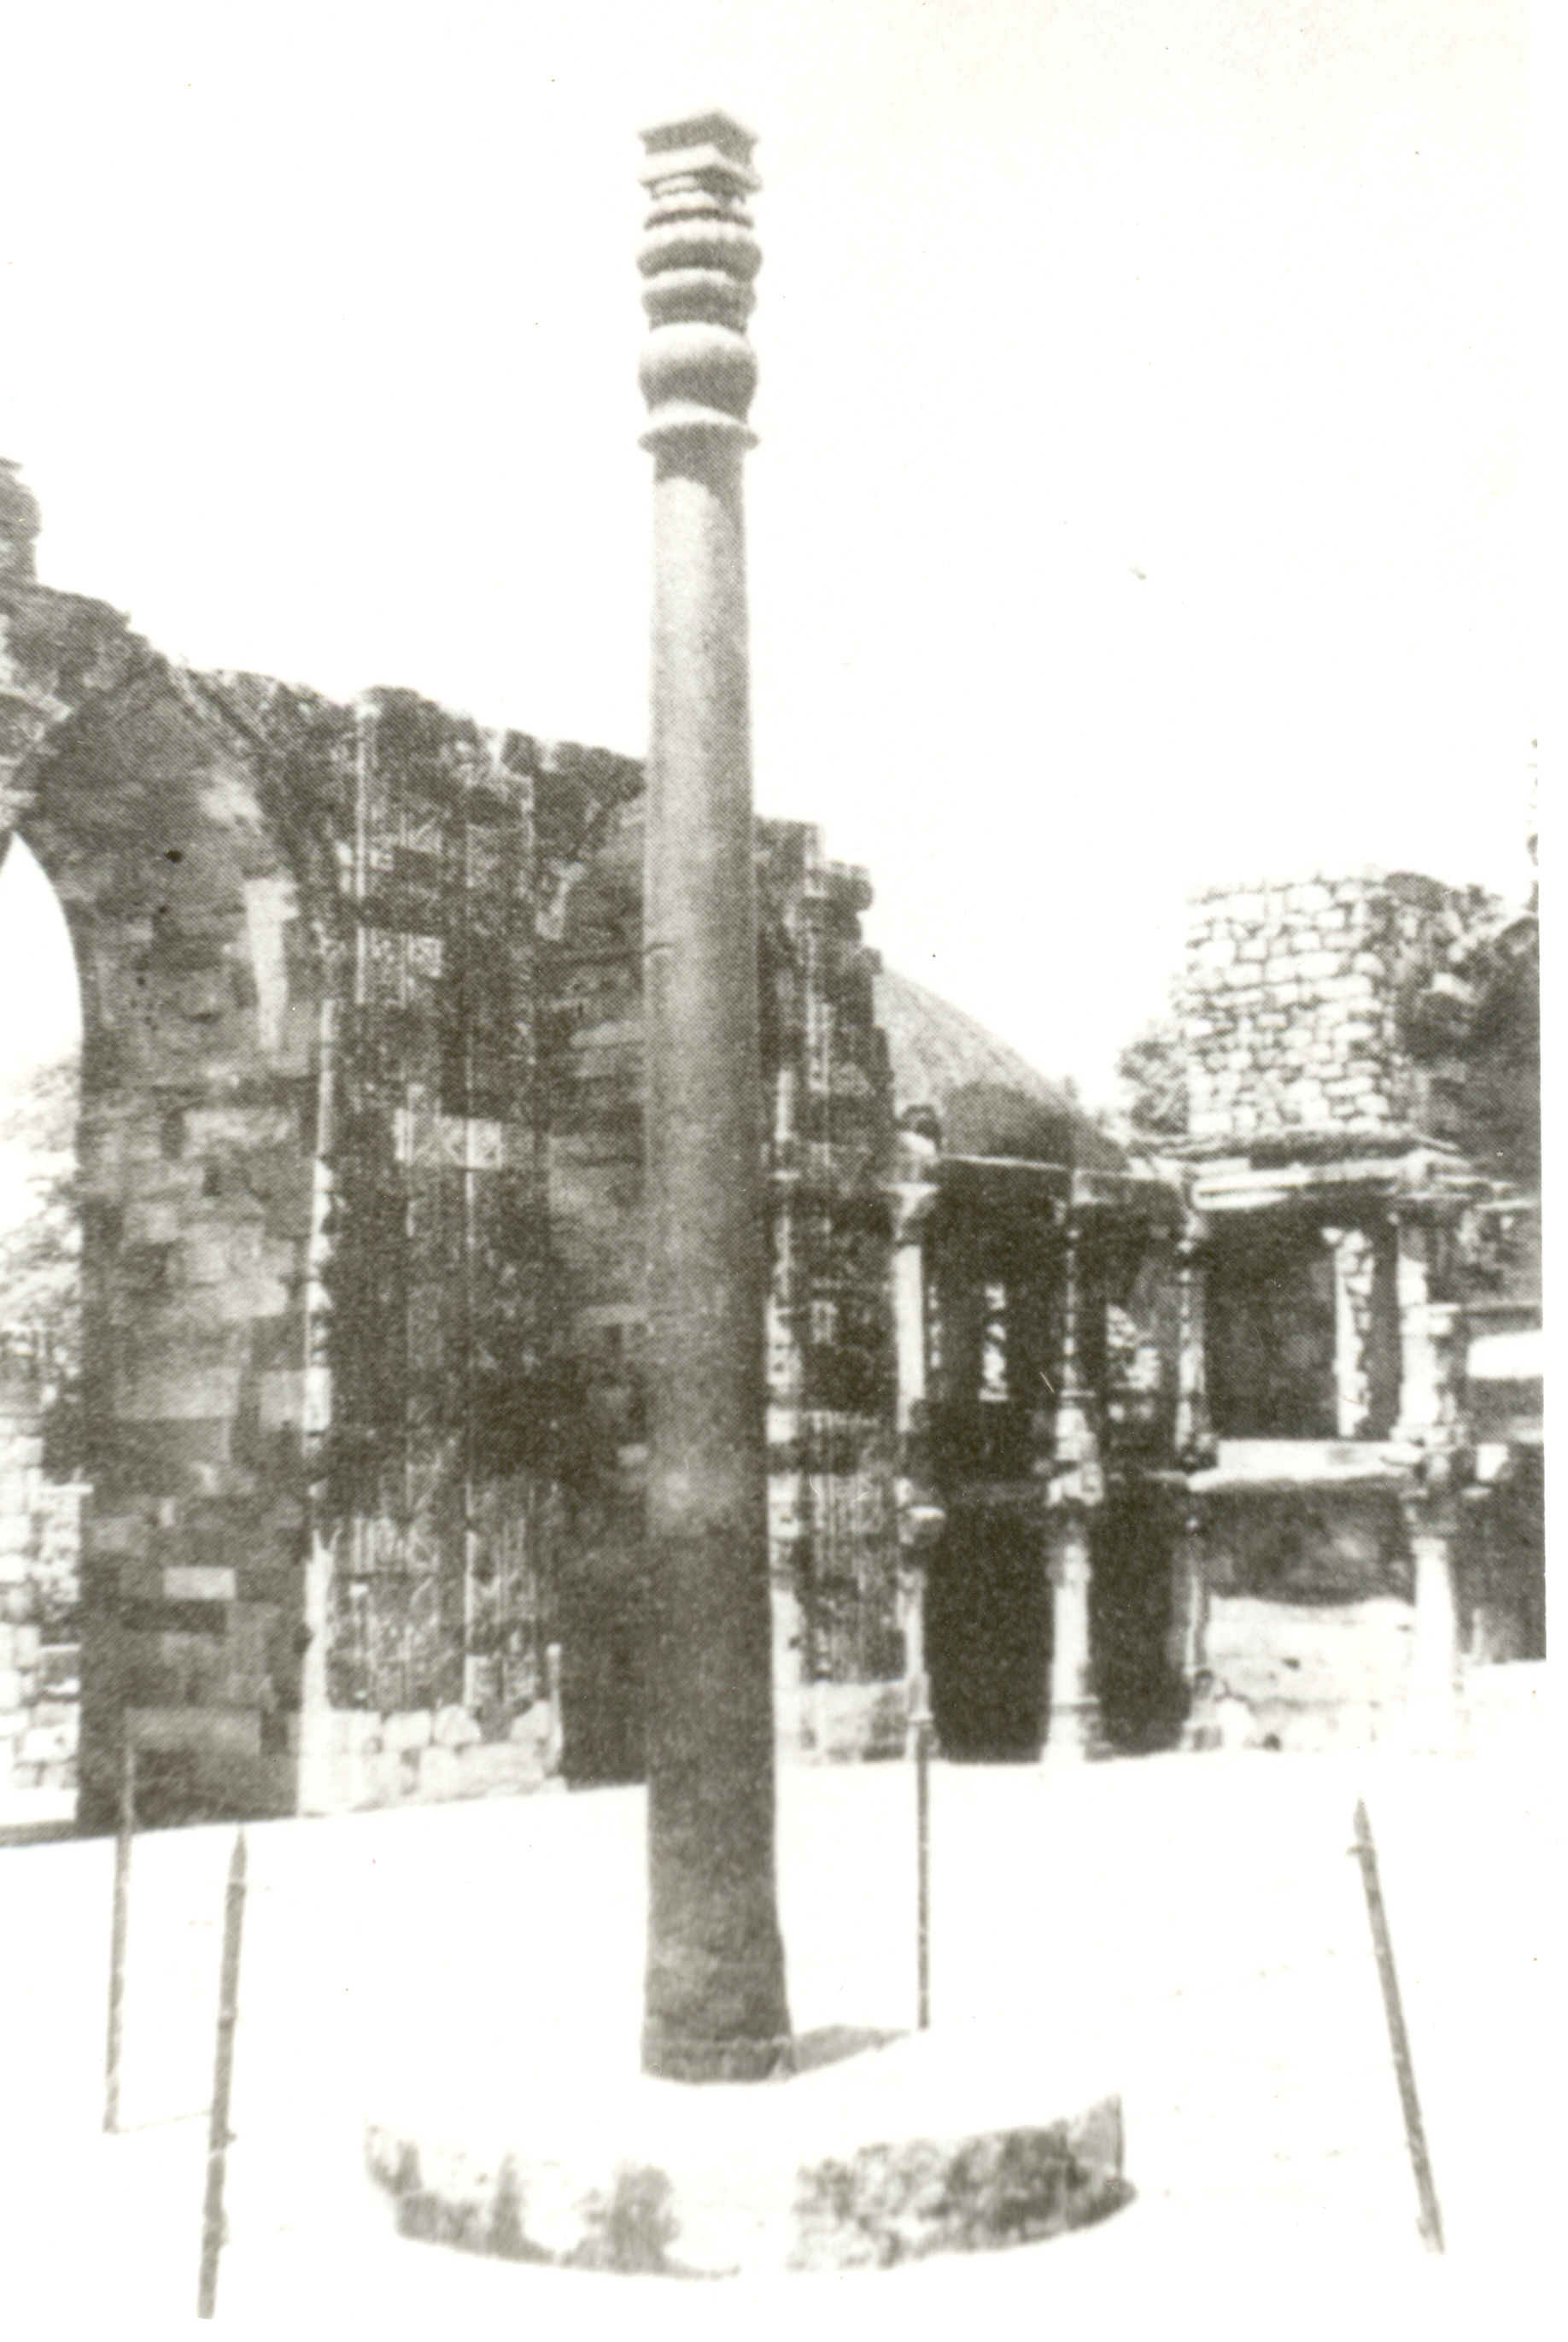
\includegraphics[scale=.3]{images/chapter-5/Fig28B.jpg}
\caption*{\textit{Fig.~28 A B Delhi Iron Pillar}}
\end{figure}

\begin{figure}[H]
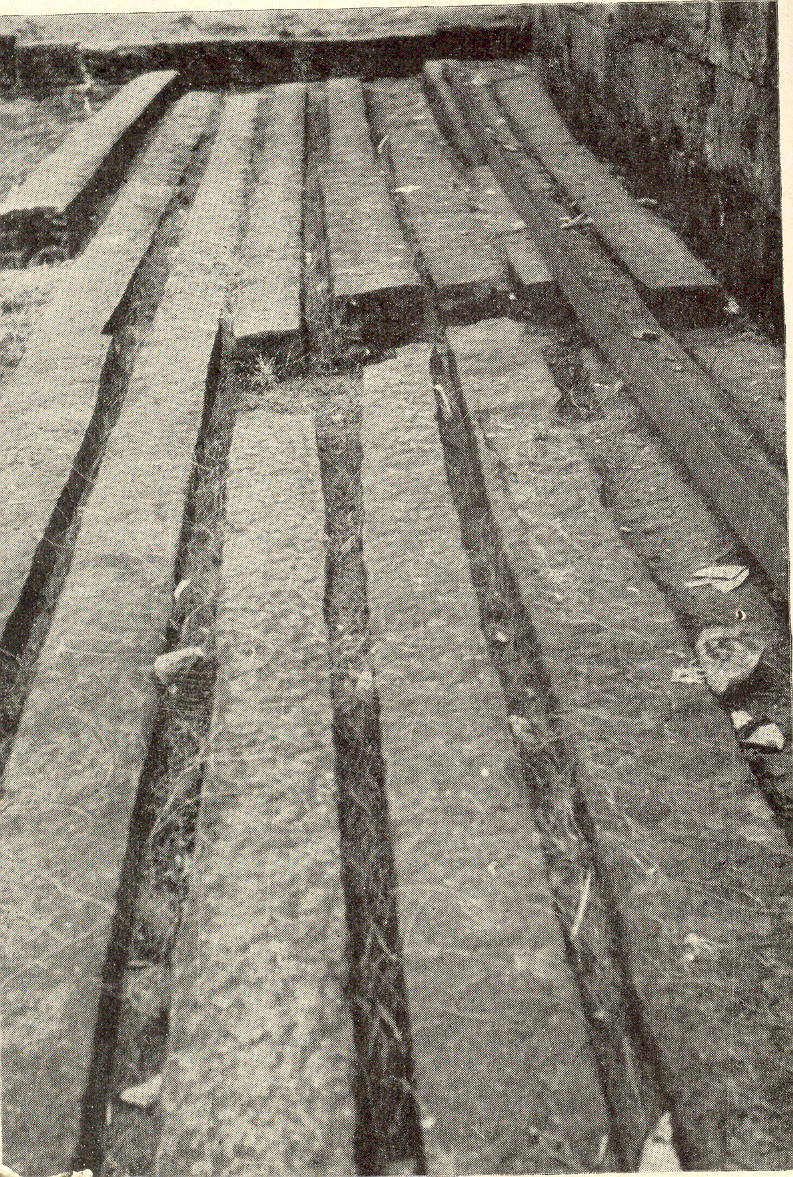
\includegraphics[scale=.7]{images/chapter-5/Fig29A.jpg}
\caption*{\textit{Fig.~29A Sun Temple}}
\end{figure}

\begin{figure}[H]
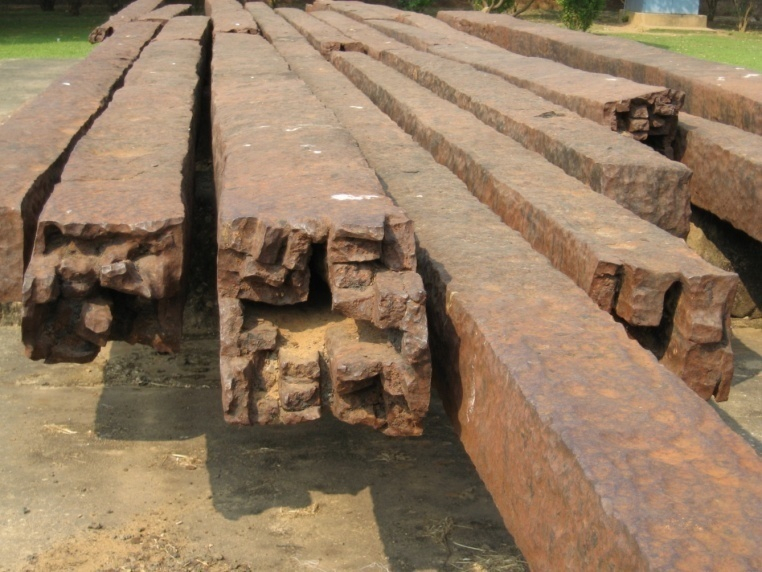
\includegraphics[scale=.7]{images/chapter-5/Fig29B.jpg}
\caption*{\textit{Fig.~29B Cross Section View of the Beams}}
\end{figure}

\noindent \textbf{\large Iron Beams at Bhubaneshwar}

The pillars described above were raised as victory monuments. But massive iron beams were fashioned to be used in constructions such as in colossal temples. An important example is that of Sun temple at Bhubaneshwar, Orissa, dated to $9^{\rm th}$ century CE. A number of such beams are lying in the temple complex even today. The largest beam weighs nearly 2721kg and is 10,668 mm long and $170 \times 190$mm in cross section  (Fig.~29). The technique adopted in their manufacture is forge welding together of thin iron bars. They manifest the expertise in forge welding that the ironworkers had mastered in the $9^{\rm th}$ century CE.

\noindent \textbf{\large The Dhar Pillar}

The iron pillar at Dhar, near Indore in M.~P., is another marvel of iron metallurgy in India. The appreciation expressed by Vincent Smith (1898) on seeing the Dhar pillar is worth quoting: 

“While we marvel at the skill shown by the ancient artificers in forging a great mass of Delhi pillar, we must give a still greater measure of admiration to the forgotten craftsmen who dealt so successfully in producing the still more ponderous iron mass of the Dhar pillar monument with its total length of 12801.6mm (Smith 1898: 143-146)”. It is the tallest iron pillar so far anywhere in the world, (13310mm) weighing about 7000 kg. The pillar is broken into three pieces.

Ancient, Dhar was the Capital of king Bhoja (1010-1053 CE.). An illustrious ruler, and a learned man. Bhoja, was said to be well versed in a rich variety of arts and crafts and a great connoisseur of art, craft, and literature. As stated above Bhoja had composed {\it Yuktikalpataru}, a text that elaborately describes iron metallurgy and techniques of manufacturing of iron and steel, especially weapons. He made references to the earlier texts on the subject, viz. {\it Lauhārnava, Lauhadsp} and {\it Lauhapradīpa}. This is significant indeed. Firstly, as noted above, it shows that iron making had developed into a well-documented science by Bhoja's times and secondly, a versatile ruler like Bhoja considered it worthwhile to compose a text on iron metallurgy. It shows the importance attributed to iron technology during that time. This suggests that the metallurgy had developed enough to be classified as a science. Texts like {\it Yuktikalpataru} or RRS along with others mentioned herein prove otherwise. 

The Dhar pillar is believed to have been originally erected in the Shiva temple of Lateshvara constructed by king Bhoja in the province of Lateshvara Mandala. When Alauddin Khilji conquered Malwa in 1399 he appointed Dilawar Khan, the Governor of Dhar who later usurped the throne and became ruler of Malwa. His son and successor Hoshangshah made it his capital. The pillar was removed in 1405 CE. to a mosque called Lat Masjid perhaps at the same site where the temple was originally located using the same architectural members. The pillars of the mosque belong to Hindu and Jain temples. Later Bahadur Shah tried to take the pillar to Gujarat. In transportation, that pillar broke into two or three pieces. Two pieces measuring 6705.6mm and 3962.4mm each have been found at Dhar. Causens (1902) mentions a third piece of the pillar somewhere in Mandu that was later brought to Dhar. Now all the three pieces lie near the modern Lat Masjid. Balasubramaniam (2002: 122-125) gives a detailed description of the history and metallurgy of this massive pillar. Another piece, that is supposedly the fourth one, is about 914.4 mm tall and currently stands in front of Jami Masjid at Mandu. The pillar is locally called Allauddin's sang (spear). It may be recalled here that it was Allauddin, the first Muslim ruler who had plundered Malwa and possibly toppled the pillar standing in front of the temple had taken away the upper portion of the pillar to be set up in the mosque complex as a trophy of his victory, and a symbol of the demolition of the temple. The pillar stands in front of the mosque. According to Balasubramaniam (op cit, 127-8) there must have been a {\it Trishul} (trident) capital on the pillar as is customary for Shiva temples. 

The pillar has been forge-welded by the horizontal forge welding technique quite similar to the Delhi Iron pillar. Roessler (1995) observed “at the bottom of the largest part there is a perimeter of 1117.6mm in the middle 1092.2mm and on top 1041.4mm, which means the square is reduced by only 121.92mm each side from the top to the bottom of the 7366mm high pillar. It shows the exactness of the forging.” For a detailed analysis of the iron of Dhar pillar, see Balasubramaniam (op.cit.) and Joshi (1970).

\textbf{The composition of iron:} Balasubramanaiam (op.cit.) reported the following composition of the iron of this pillar - 55.8\% Fe, 27. 8\%. Si, 0.1\%. Mn, and 16.3\% P. He specially underlines the high proportion of phosphorous in Dhar pillar as is typical in ancient Indian iron. The corrosion resistance of such iron is attributed to this factor. Suffice it to comment here that the Dhar pillar is the tallest and heaviest (7000 tons) iron pillar anywhere in the world even though it belongs to such an early date. It is a tribute to the master artisans of the period.

\noindent \textbf{\large Iron Pillar At Kodachari Hill}

Another iron pillar of pre-modern period may be noted at the Mookambika temple at Kodachari hill. According to Anantaraman (1999) it may have been a flagstaff of a temple. The place Kodachari is located at about 40 km from Kallur, 120 km north of Mangalore, Karnataka. It is 10058.4mm high pillar with a rectangular cross section (86.36mm x 58.42mm). Anantharaman, on the basis of XRD analysis, finds it to be of pure iron with small percentage of carbon. The microstructure shows ferrite with small percentage of pearlite in it. The date and historical significance of the pillar at Kodachari are not clear except for the fact that Anantraman felt that it is a pre-modern product with reddish protective rust indicating a process of protective rust formation similar to that of Delhi iron pillar.

\noindent \textbf{\large Iron Pillar at Mount Abu}

A 3886.2mm tall iron pillar stands in the Achaleshwar temple at Mount Abu. Neogi (1914) dates it to 1412 CE. It is a pillar with a trident ({\it Trishul}) at top as its capital. Very little has been written about it except that Cousens (1902) noted that it was erected to commemorate the victory of the Hindu ruler over the Muslim forces of Alauddin Khilji. However, it goes to prove that massive structures of iron continued to be manufactured right up to $15^{\rm th}$ century CE, or possibly even later. It proves without doubt that the infrastructure, technology and work force of metal workers were still vibrant. Indeed, a large network with organizational set up was an essential feature for such massive monumental structures of metal. It was followed by a phase of Moghul war weapon manufacturing. The imperial Moghuls appear to have readily tapped the infrastructural facilities that existed at that time.

It has generally been argued that metallurgy in ancient India was more of a craft based on experimental foundations of a practicing class. Sabyasachi Bhattacharya (2002) posed the question “...what was the element of scientific knowledge in the production of such superior artifacts (Delhi iron pillar) and did India lose that knowledge in course of time?" Buchanan during his surveys of eastern India in the districts of Patna, Gaya, Shahabad etc. during the years 1810 to 1813 commented on the absence of scientific or theoretical basis of iron metallurgy (especially in eastern India). Similarly, Voysey in 1820 CE met Persian merchants at Konasamudram who had come there to buy steel for the production of swords; but the artisans according to him had no theoretical knowledge of the technique that they practiced.We have already brought up this issue above. The following points go against such an assumption:

\begin{enumerate}
\item Bhoja produced a text, Yuktikalpataru– on iron making. In addition to his own composition, he also referred to the texts on metallurgical science (mentioned above) which were written before him by masters on this subject. It is most unfortunate that these treatises on iron metallurgy are now lost.
\item The other observation is that the scientific principles were totally absorbed and turned into a technology in our society, which was well adept in oral and verbal transmission of knowledge.
\item There are two distinct classes perceptible in the Indian social system 
\begin{enumerate}
\item the Brahmans or the theoreticians, and 
\item the working class who translated that knowledge into practice. Mostly this was practiced under the able guidance of the former.
\end{enumerate}
\item The loss of theory could also be attributed to two factors:
\begin{enumerate}
\item Prolonged political turmoil and devastation of intellectual tradition and property that has been mentioned by medieval period records. It is a well recorded fact that the libraries at Taxila, Nalanda, Vikramshila and several educational centres which had been attracting scholars from across the world were burnt down. The looting and plundering by the early Mohammedan invaders targeted not only temples and monasteries for their riches but had destroyed the science and technology which was being taught there.
\item The knowledge on various subjects was also kept secret by masters. Such secretive attitude of the artisan class was also responsible for loss of know how. If something went wrong, the knowledge died with the masters. 
\end{enumerate}
\end{enumerate}

\section*{The Mighty Moghuls}\label{chapter5-section-2}

The Moghul period of Indian history is well known for its prosperity and affluence. The Moghul monuments in India speak of the glory and wealth of that period. The ruling class, the nobility and officials of the state of Moghul India led a luxurious life. The wealth was generated by an organized economic system the state. Trade, commerce, industry and agriculture were highly productive. Babur, on his arrival noted that the good things that could be said of `Hindustan' was that it had `unnumbered and endless workmen of every kind' ({\it Baburnama}\endnote{Baburnama or Tuzuk-i-Baburi, Turki text edited by A.S. Beveridge London, 1905, Translated by J. Leyden and W. Erskine revised by L. King Oxford 1921. A.S. Beveridge London 1921 (Delhi edition 1970)}, 168; II). It clearly testifies to the presence of a highly productive craft and variety of skills. The workmen excelled in industry. A sizeable population was engaged in these activities. It is apparent therefore that though texts on scientific knowledge had been generally lost and a decline had set in by $13^{\rm th}$ –$14^{\rm th}$ century, the tradition had survived with the artisan class. Their number and diversification had thus surprised the Moghuls as evident from the statement made by Babur. It was this class of `unnumbered and endless workmen' that must have been the backbone of the Indian economy. Our focus here is the iron working and the class engaged in smelting, forging and smithy of iron during the Moghul period.

Regarding the basic nature and technique of iron production, there is little evidence to suggest change or innovation. The same old clay furnaces operated through foot bellows continued. The labour intensive iron industry of the earlier times remained the norm even during the Moghul period, as will be discussed a little later. However, with growing emphasis on arms and armours there arose the requirement of iron for their production on a much larger scale. This must have naturally led to better organization of the industry. A larger number of artisans were commissioned to produce more and more iron at individual or family levels. Simultaneously, foundries or {\it Shahi Karkhanas} became busier as they operated in a highly organized fashion. They must have employed the skilled ironworkers for the manufacture of firearms that were required as also the huge cannons the Moghuls were extremely fond of. The emperors themselves took personal interest in their design and manufacture. Presumably gun casting had started in India earlier (circa 1400-1500 CE), before the arrival of the Moghuls as has been argued by several scholars of medieval history (Jaggi 1989: 125-127). Among the centres of manufacture for guns, special mention has been made of Gujarat and Deccan. Both these regions were known for their excellent iron production centers. They had also exported steel for a long time. No wonder that they continued the tradition later on as well.

\vspace{-.3cm}

\subsection*{The Iron Cannons}\label{chapter5-subsection-2.1}

\vspace{-.2cm}

 It is believed that the first cannons roared in India during the battle of Panipat in 1526. They were fired by the Moghul forces of Babur, the first ruler of a dynasty that ruled the country for several centuries. However, there is controversy on the earliest use of cannons (Jaggi 1989: 126-128). Some medieval records including that of Barni mention the use of firearms and cannons from the $13^{\rm th}$ century onwards. According to Joshi (1970), P.K. Gode in an article, `Use of guns and gunpowder', affirmed the use of guns and gunpowder from 1400 CE onwards. A Chinese traveler called Mahum who visited Bengal in 1406 CE mentioned the use of guns there. There are also references of its use in Kashmir by 1466 CE and in Gujarat in 1482  CE. The Sanskrit text on polity {\it Shukraniti} dated roughly around 1600  CE mentions two types of firearms used in its times, viz., {\it Kshudra nalika} (small guns or match locks) and Brihad nalika (large guns or cannon). Their measurements have also been specified to be 409mm long having a longitudinal bore of thickness of the middle finger and provided with two raised points for taking aim. The {\it Brihad nalika} were moved on carriages and their range depended on the thickness of the metal plates.

%~ \newpage
However, the Moghuls were the major users of cannons and continued to manufacture them for centuries. Moghuls attached great importance to artillery. {\it Ain-e-Akbari} boasts that `excepting Rum (ancient Turkey) no kingdom could compare with the Indian empire under the Moghuls in the number and variety of weapons'. They had a full-fledged establishment to look after it. Though some of the heavy guns made more noise than caused damage, they must have been a terror at that age. There are a large number of such cannons adorning the important buildings today, which have not been systematically recorded or studied so far. 

Neogi (op. cit.) describes two types of cannons used during the mediaeval ages - those bearing the inscription in Persian - {\it taiyar shud} (one that was manufactured by forging) and the other {\it rekhta shud} (one that was cast). The latter must have been bronze cannons that were being cast and the former were of wrought iron. Several wrought iron cannons have been mentioned in great detail in literature, e.g. a 7010.4mm long piece designated ‘Kaley Khan’, and a 5334 mm long and 1600.2 mm diameter gun. At Murshidabad a cannon called ‘Jahankosh’ (conqueror of the world) was constructed in 1637 CE during Shahjahan’s reign. There were other cannons like the 7315.2mm long iron cannon at Nurvar, the ‘Landa Kesab’ and {\it ‘fire flier’} at Bijapur, also one at Gulbarga, and the often-mentioned cannon at Tanjavur (Plates, fig.30-39).


\begin{figure}[H]
\setcounter{figure}{29}
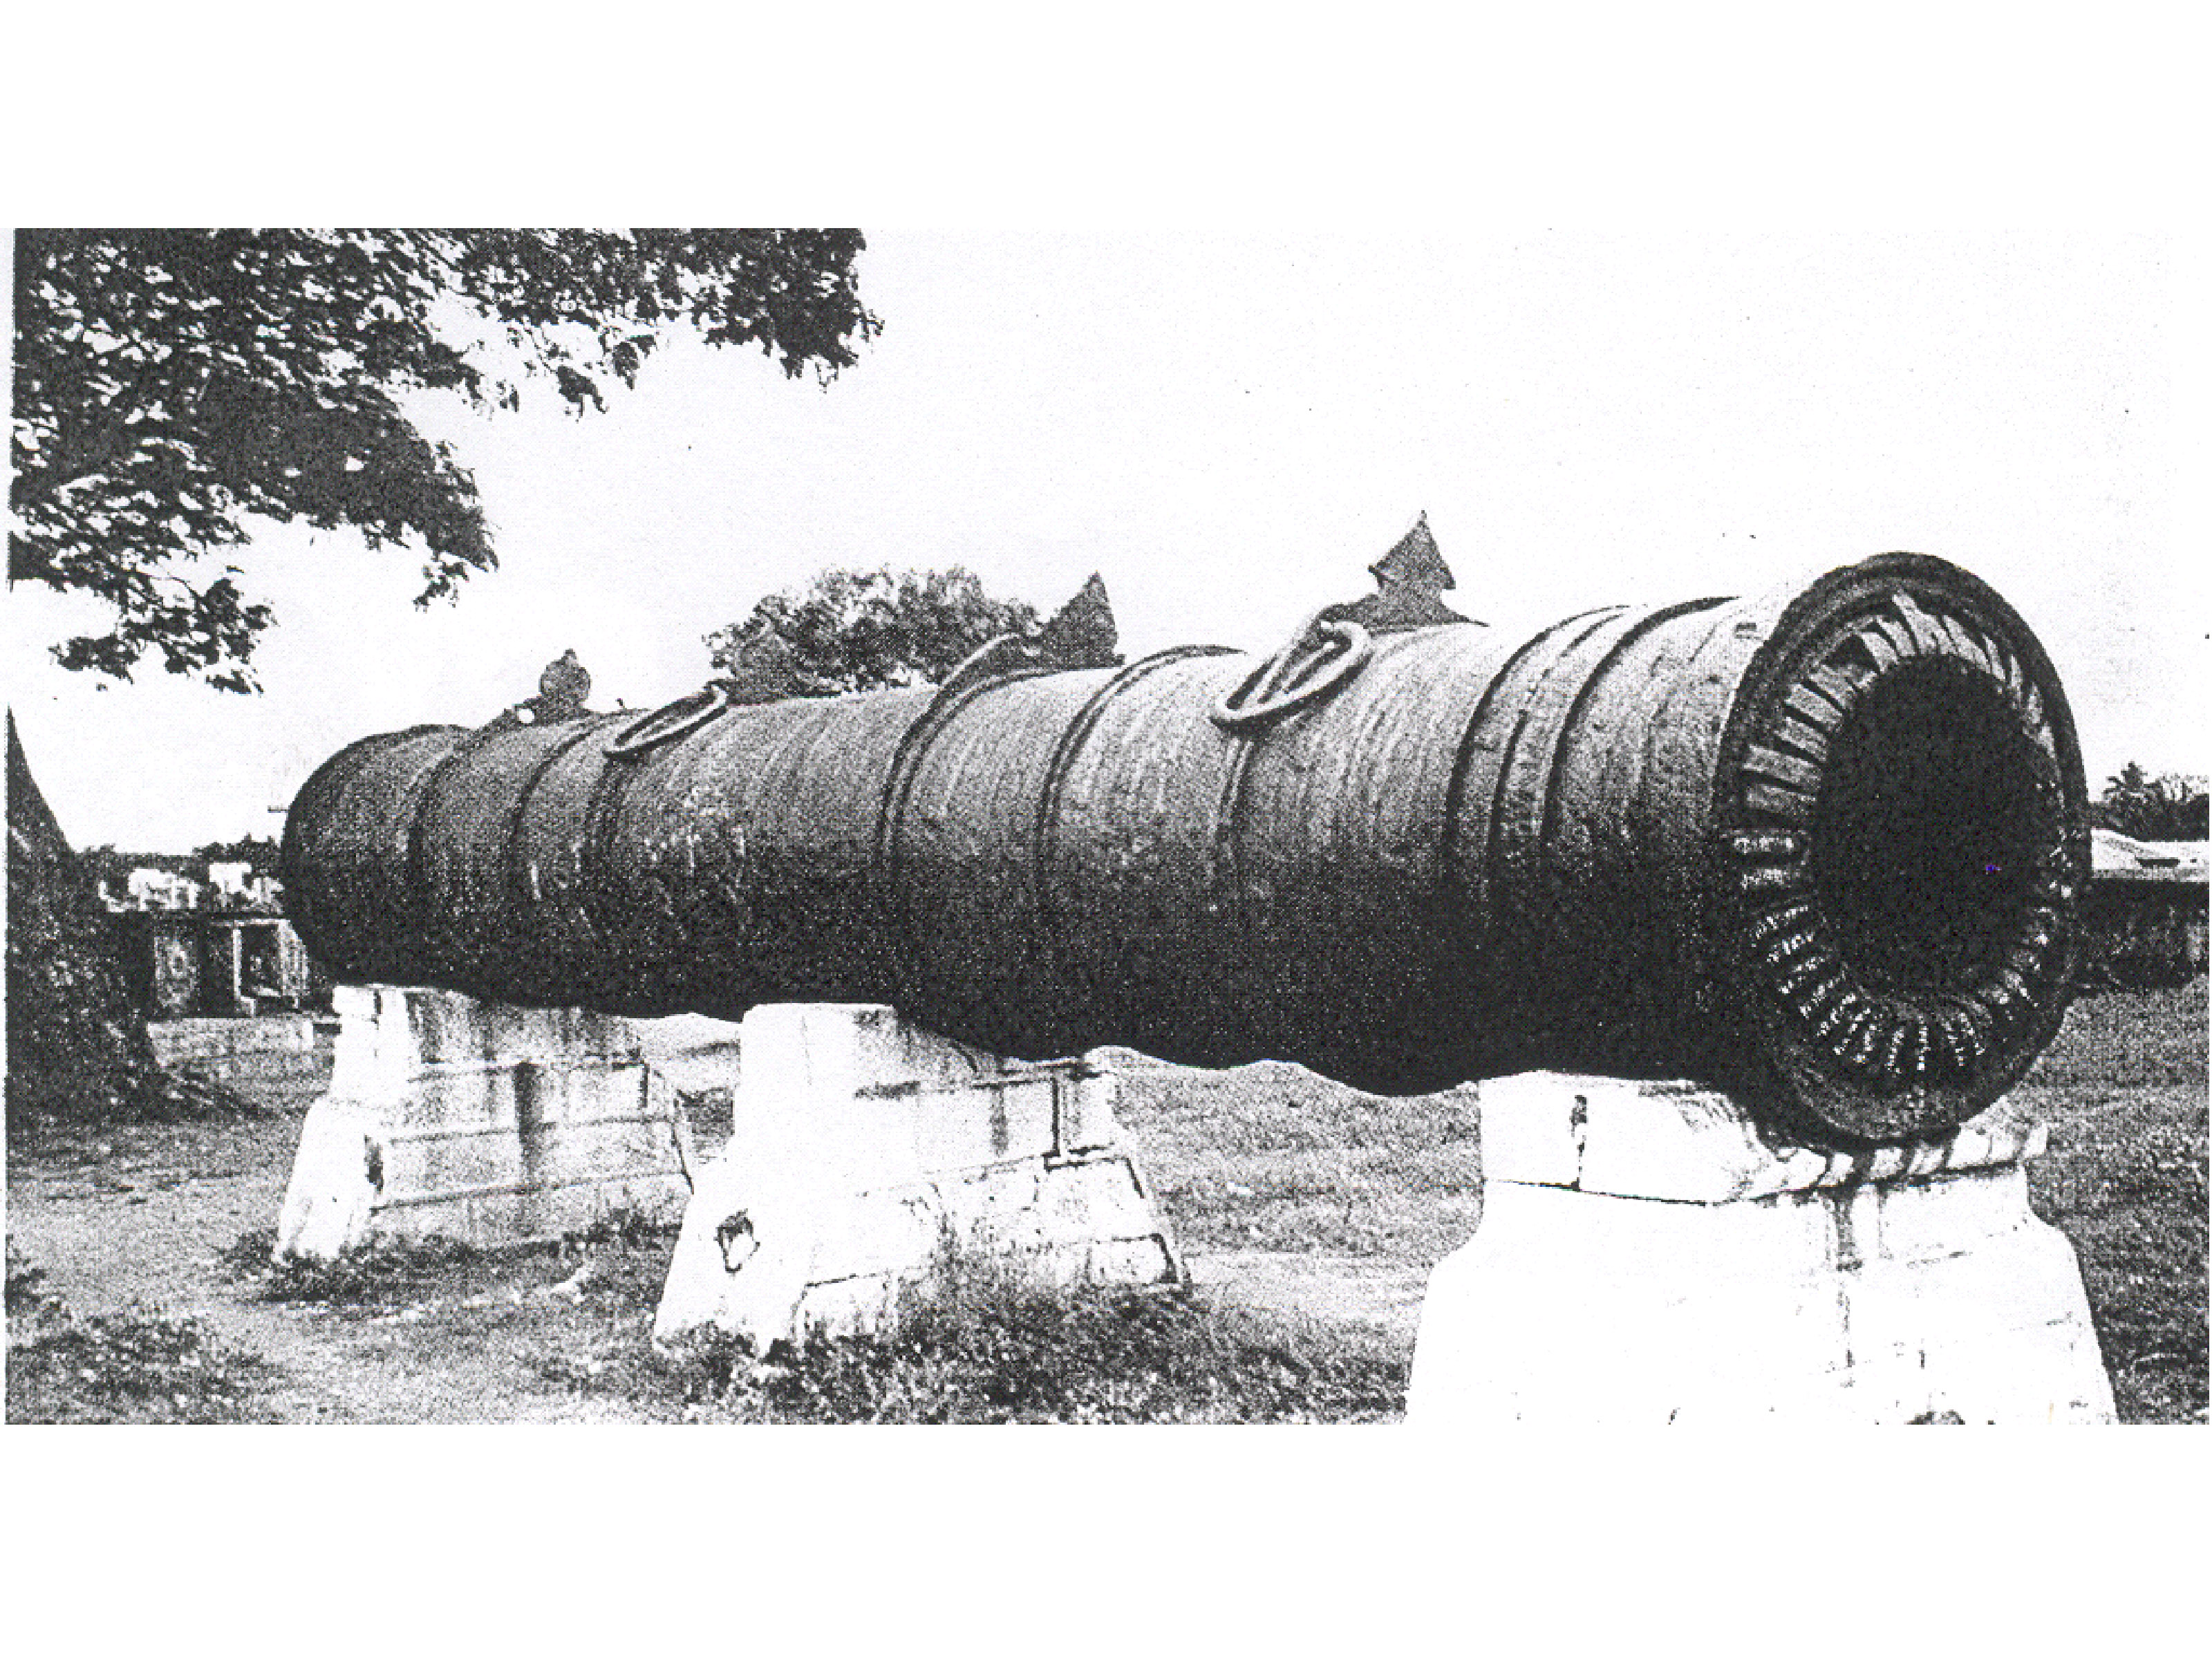
\includegraphics[scale=.7]{images/chapter-5/Fig30.jpg}
\caption{\textit{Cannon Tanjavur fort}}\label{chapter-5-fig30}
\end{figure}
\begin{figure}[H]
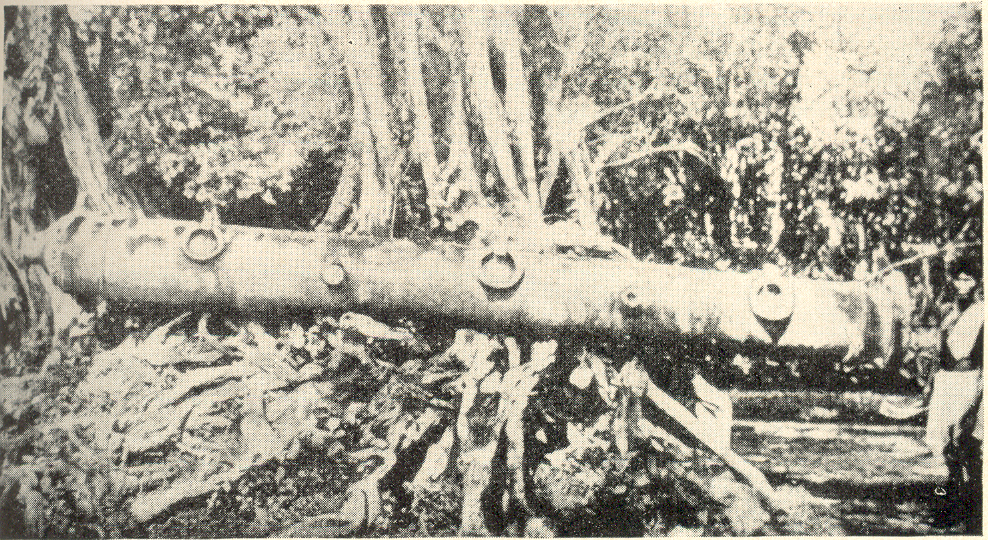
\includegraphics[scale=.7]{images/chapter-5/Fig31.jpg}
\caption{\textit{Jahankosh, Murshidabad}}\label{chapter-5-fig31}
\end{figure}
\newpage
\begin{figure}[H]
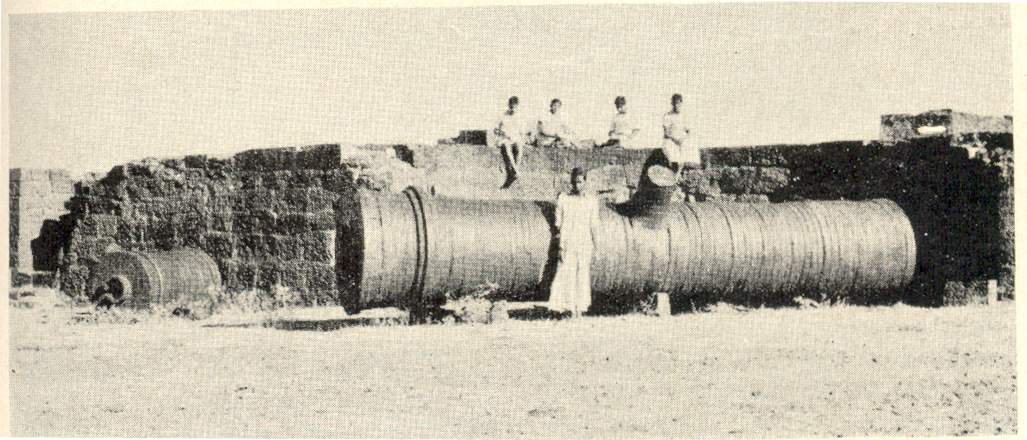
\includegraphics[scale=.7]{images/chapter-5/Fig32.jpg}
\caption{\textit{Cannon - Landa Kasab, Bijapur}}\label{chapter-5-fig32}
\end{figure}
\begin{figure}[H]
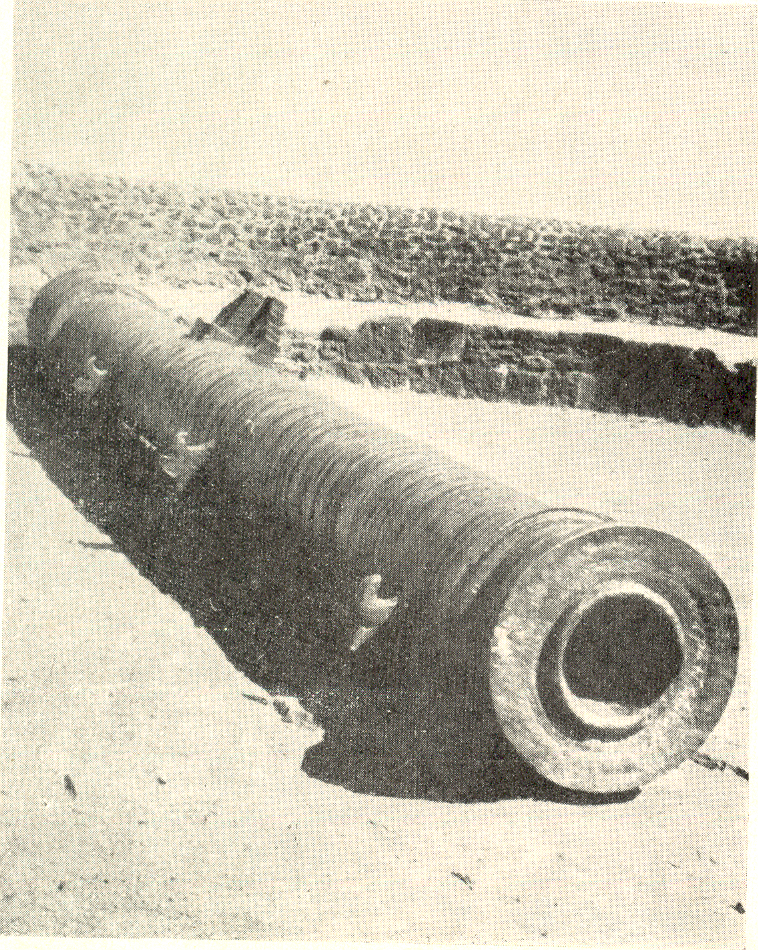
\includegraphics[scale=.7]{images/chapter-5/Fig33.jpg}
\caption{\textit{Far flier, Bijapur}}\label{chapter-5-fig33}
\end{figure}

\newpage

\begin{figure}[H]
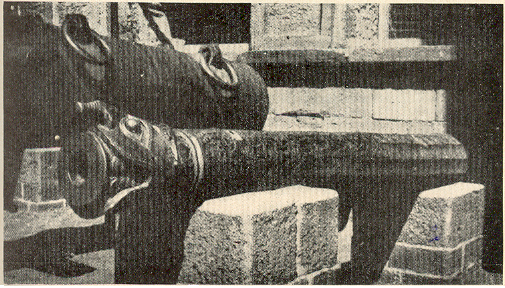
\includegraphics[scale=.7]{images/chapter-5/Fig34.jpg}
\caption{\textit{Gemda Top, Cannon of Aurangzeb, Bijapur}}\label{chapter-5-fig34}
\end{figure}
\begin{figure}[H]
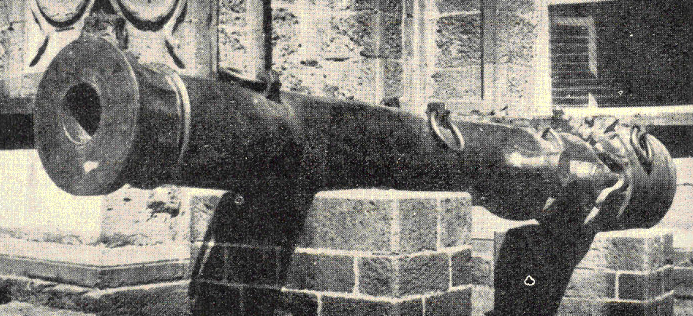
\includegraphics[scale=3]{images/chapter-5/Fig35.jpg}
\caption{\textit{Cannon with alligator shaped barrel, Bijapur}}\label{chapter-5-fig35}
\end{figure}
\begin{figure}[H]
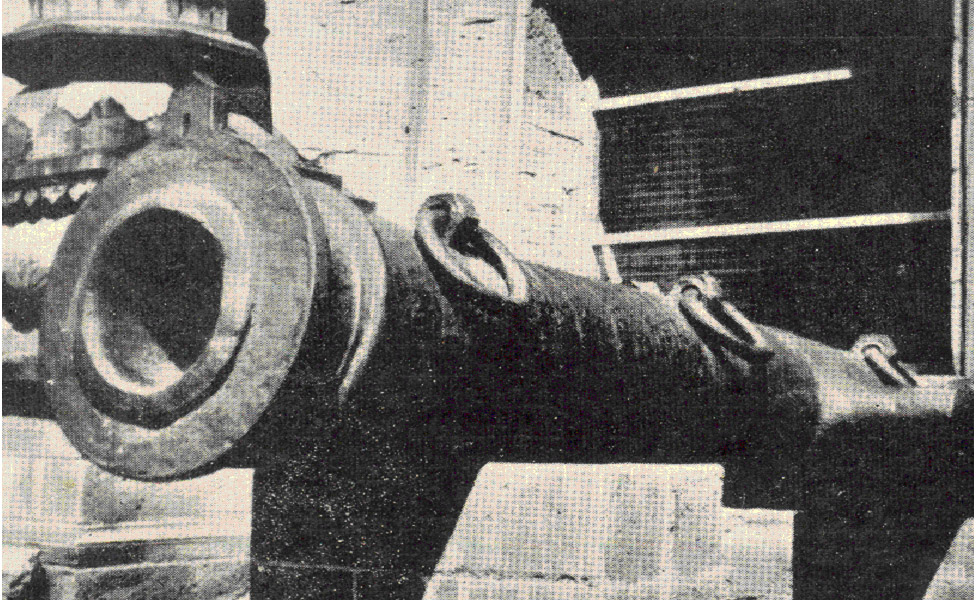
\includegraphics[scale=1.2]{images/chapter-5/Fig36.jpg}
\caption{\textit{Panj-mani-Adil-Shahi Ahmed Burj, Bijapur}}\label{chapter-5-fig36}
\end{figure}

\newpage

\begin{figure}[H]
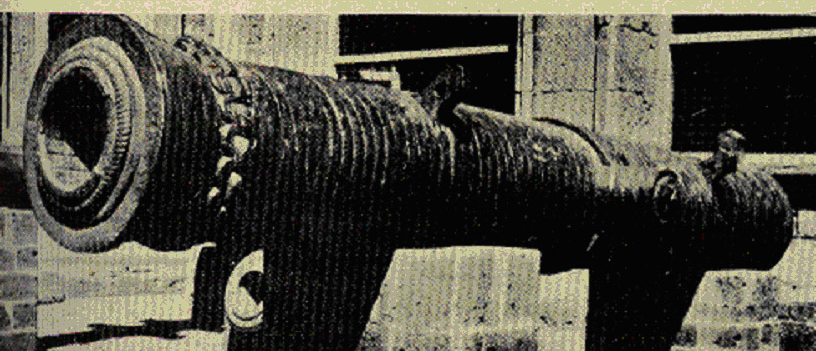
\includegraphics[scale=1.2]{images/chapter-5/Fig37.jpg}
\caption{\textit{Cannon from Malik-Sandal Burj, Bijapur}}\label{chapter-5-fig37}
\end{figure}
\begin{figure}[H]
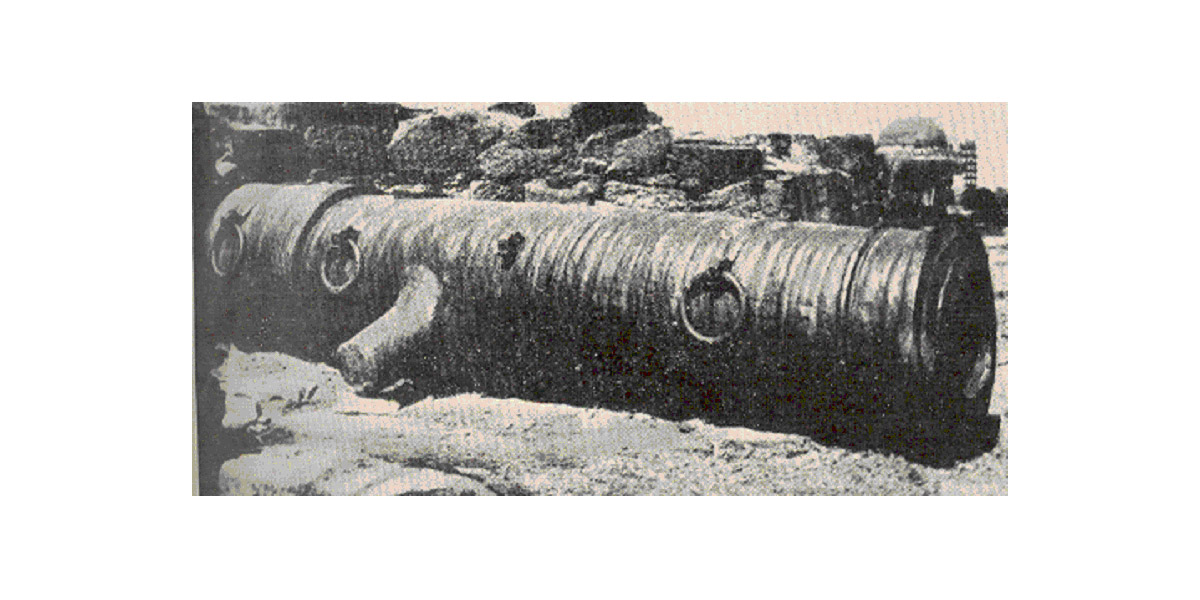
\includegraphics[scale=1.2]{images/chapter-5/Fig38.jpg}\label{chapter-5-fig38}
\caption{\textit{Golgumbaz, Bijapur}}
\end{figure}
\begin{figure}[H]
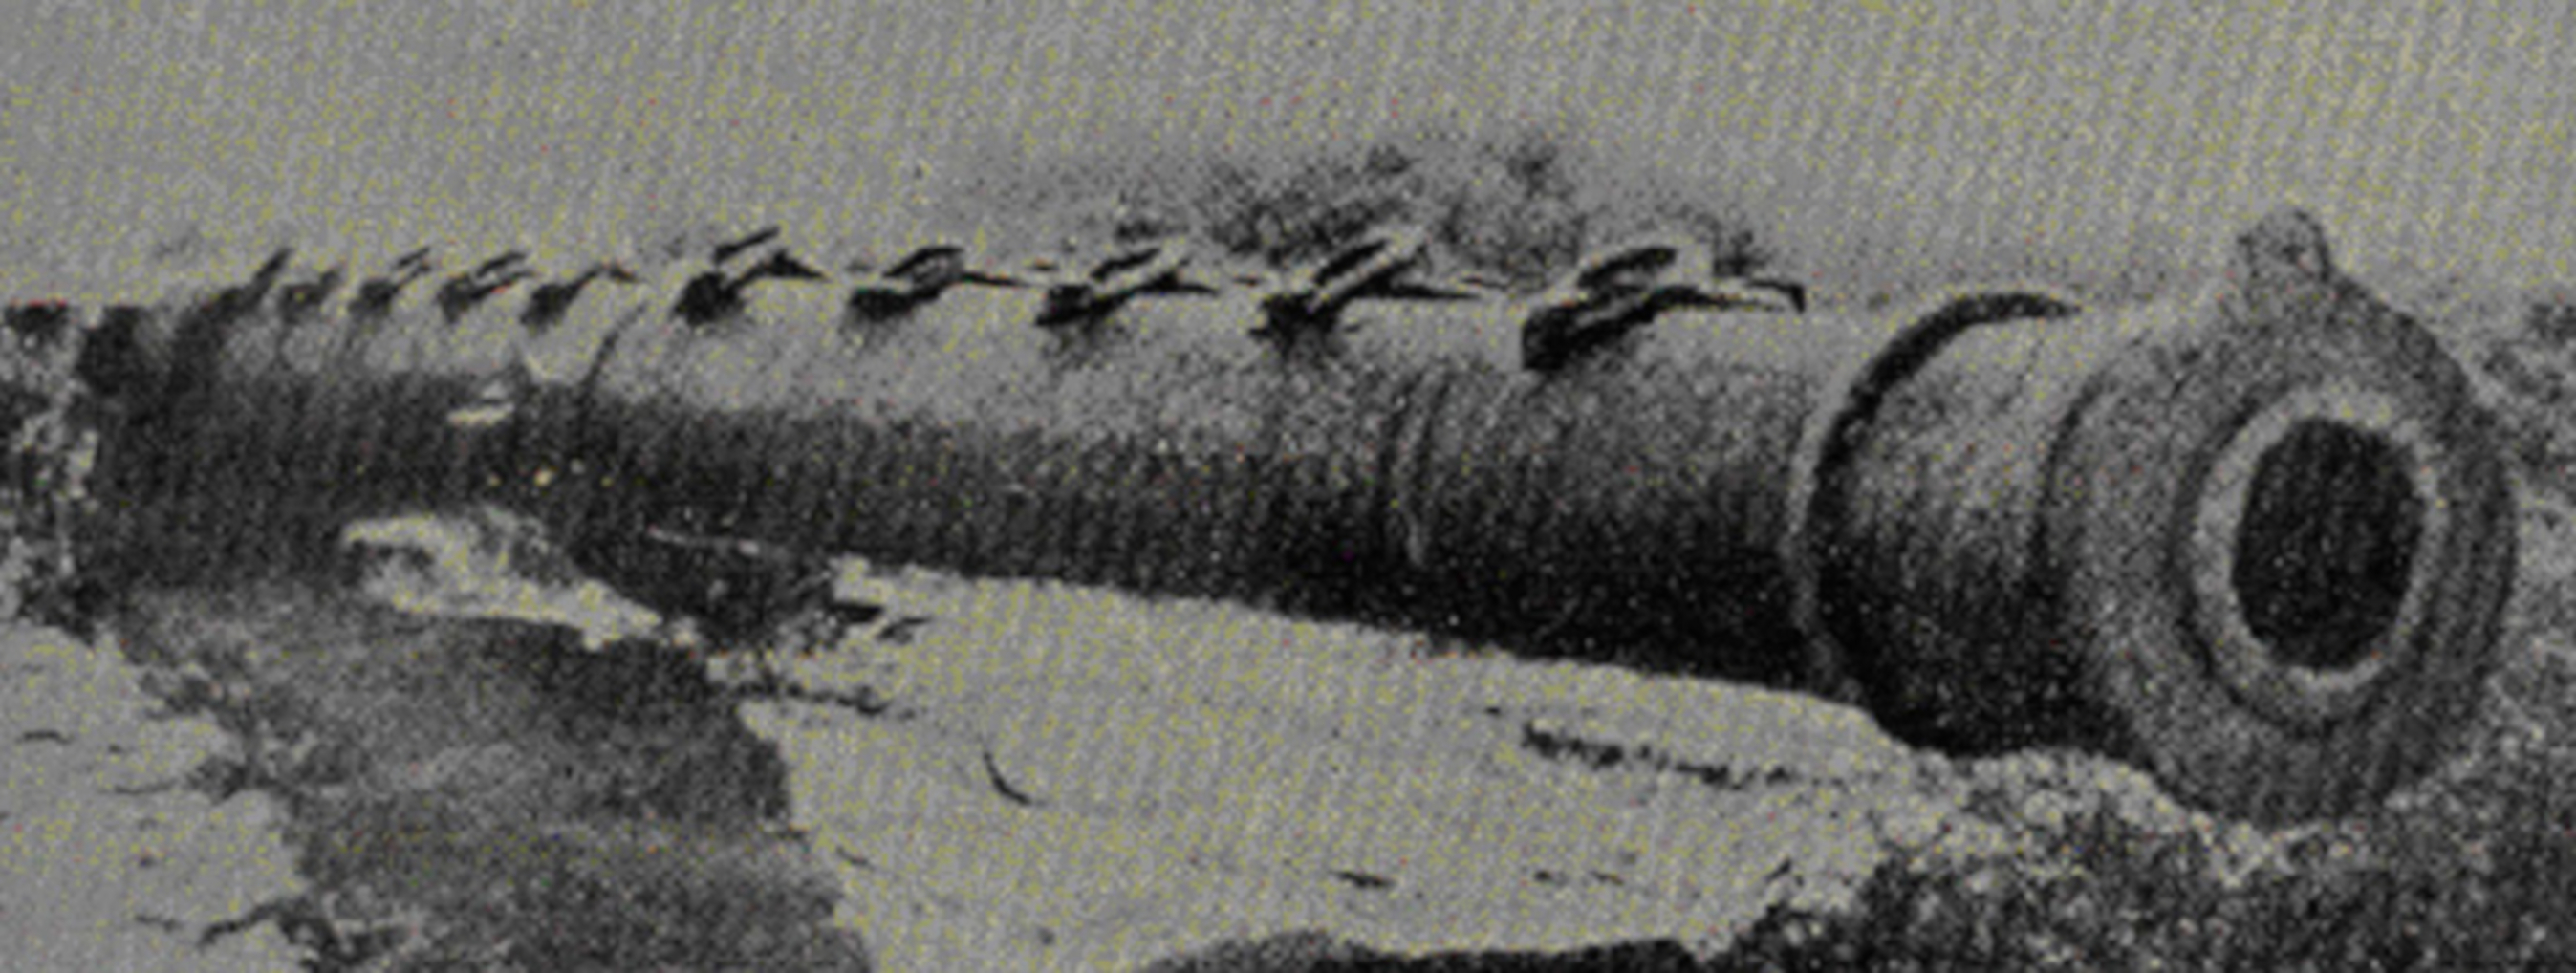
\includegraphics[scale=1.2]{images/chapter-5/Fig39.jpg}
\caption{\textit{Cannon at Gulbarga, Karanataka}}\label{chapter-5-fig39}
\end{figure}

Once firearms like cannons and guns came to be manufactured with iron replacing the earlier bronze weapons, the demand for iron must have increased. At the same time experts were invited from the Middle Eastern countries to assist in manufacturing of weapons. Akbar’s foundry establishment was managed efficiently by one Amir Fathaullah (1564-90) who is said to be a well known expert in mechanical tools. He hailed from Shiraz in Persia and was invited initially by Adil Shah of Bijapur. He later joined the Shahi arsenal.

The iron cannons were manufactured with longitudinal iron bars welded together with circular rings shrunk fit on them. Special mention may be made here of the cannon at Thanjavur (fort) (Fig.~30). It has been studied in great detail by Roessler (1997). The inner bore of this gun has been made by placing iron rods parallel to each other and fixing them together by a series of iron rings (Fig.~30). It is 8077mm long. The external diameter is 1117mm and internal one of 638mm bore. It weighs approximately 35400kg though there are a large number of such guns but an in-depth and detailed metallurgical study of cannons and other weapons manufactured during the Moghul rule is yet to be undertaken. However, it is certain that steel production was more centralized and better organized during this period. There must have been a greater state control as may easily be deduced from records of this period. We may come back to this issue, a little later.

``Under Emperor Akbar, the artillery attained greater efficiency. With the technical help of Fathullah Shirazi, after he joined Akbar’s court in CE 1583, many innovations were carried out which included making a machine for cleansing gun barrels, portable cannons, multi-barrel cannons, etc.” (Jaggi~op.~cit.~p.~130). A good example is that of innovative design of a gun-barrel-cleaning machine. The idea behind developing it was to use bullocks, thereby relieving men for fighting or other important jobs. The machine cleaned 16 barrels at the same time. ``It was worked by a bullock, its movement, as in an oil press, rotated the axle, which in turn rotated the brush rod inside the barrel, through the movement of the cogwheel and pinions. The portable cannon was developed to facilitate the movement of the heavy artillery to hilltops.~The entire cannon was fabricated in parts, each part being then screwed to the other. It could be easily dismantled or assembled as and when required and could provide greater mobility to the heavy artillery. There were a number of such cannons in use at the time of Akbar. The multi-barrelled cannon was developed by welding these pieces in a row; it could be fired in quick succession with one match cord. These machines, in all probability, were constructed in the workshops ({\it kārkhānās}) of the emperor. These workshops were well-equipped, with skilled workers, who were attracted from all over the empire" (Jaggi op. cit. p.130).

The {\it Ain-e-Akbari} gives a detailed account of gun making and the types of guns being made, including the problems and defects and the precision issues. The royal arms and armours were decorated and embossed with gold and silver and occasionally calligraphed, giving details of the weight of raw and finished iron, and the place of origin of iron. The name of the artisan and the place and date of manufacture etc. were carved also on the guns. A considerable amount of attention was paid to weapon manufacturing. The Ain-e-Akbari (1, 120-21) describes methods of gun making that had been devised by the ingenuity of the emperor himself. The emperor had the iron flattened and rolled up like a scroll of paper in a slanting fashion and every fold was passed through the fire. There was also another method: solid iron pieces were properly tempered and then bored with an iron borer; and three or four of these were joined together to form a gun ({\it bandook}). Iron was made into cylindrical pieces. They were pierced with iron pins when still hot. Three or four such pieces made one gun. 

``From the practical knowledge of his Majesty, guns are now made in such a manner that they can be fired off, without a match, by a slight movement of the cock.” He also trained and produced gun makers like Ustad Kabir and Husayan. Fathaullah Shirazi devised even a ‘screw cannon’, which could be conveniently assembled at the site. About 77 weapons were listed in Ain-e-Akbari. Even their drawings are given. The details include right from the mining of ores and the amount required, smelting and manufacturing technique etc. Royal Karkhanas were the centers for producing these weapons. They were also purchased from outside when the requirement was too large. Indeed this must have been a flourishing industry during Akbar’s times.

“The {\it Ain-e-Akbari} (Moreland 1923) also provides an exhaustive list of weapons in the Moghul arsenal. The {\it Ain-i-Akbari} (1.117) gives the following long list of the various weapons in Akbar’s arsenal.  Some of these names can be recognized, others not: Swords (slightly bent), {\it Khādā} (straight swords), Guptiacā (a sword in a walking stick), {\it Jamdhar} (a broad dagger), {\it Khanjar, Khapwa, Jan Khāk, Bāk, Jhanbwa, Katāra, Narsink moth, Kaman (bows), Takhsh Kamān, Nāwak,} Arrows per bundle, {\it Quivers, Dadi, Tirbardār} (arrow drawers), {\it Paikankash, Neza} (a lance), {\it Barcha, Sāk, Sainthi, Salera, Gurz} (a war club), {\it Shashpar} (a war club) {\it Kestan, Tabar} (a war axe), {\it Piyazi} (a club), {\it Zāghnol} (a pointed axe), {\it Chakar- basola, Tabar Zāghnal, Tarangāla, Kārd} (a knife), {\it Gupti Kārd, Qamchi Kārd, Chaqu} (a clasp knife), {\it Kamān-i-Guraha} (bullet bow), {\it Kamtha, Tufak-i- dehan} (a tube), {\it Pushtkhār, Shahtawez} (has a hook), {\it Girikushā, Khār-i- mahi, Gobham} (a sling), {\it Gujbāg, Sipar} (a shield), {\it Dhal, Khera, Pahri, Udāna, Dabulgha, Khaghi, Zirih Kūlah, Ghughuwa, Jaibāh, Zirih,  Bagtar,  Josan, Char aina, Kothi, Sādiqi, Angirkha, Bhanju, (hihrah zirih-i-ahani), Salhqaba, Dastwana, Rāk (rāg,) Kantha sabha} (a neck piece of armour), {\it Moza yi- ahani, Kajem, Artak} (the {\it quilt}){\it -u-Kajem, Qashqa, Gardani} (to protect chest of the horse), {\it Match-locks, Ban} (rockets).

“The Mughal emperors with their fondness of firearms used to give grand names to their guns that suggested power and might. Some of the great guns of Aurangzeb had names such as the following: {\it Aurang- bar} (Strength-of-the-throne), {\it Kale Khan, Bijli pasand, Bandkushao} (Cruel- killer) {\it Daldali, Fat-i-laskhar} (Army-victor), {\it Hathi-.thal, Daulat-i-maidan, Malik-i-maidan, Jang-awar, Sitam} (Punisher),{\it Dilawar} (Lively), {\it Shah- inayat} (Royal gift),{\it Daim-Kushad} (Wide-mouthed), {\it Tirkhor, Burj-Shikan} (Bastion-breaker), {\it Nasir-abi} (Conqueror-in-water), {\it Shah Daultat} (Royal- riches), {\it Sar-Kushadah} (Wide-headed), {\it Nishan-i-rast} (Straight-hitter), {\it Be-khata} (Faultless), {\it Zafar-i-mulk} (Conquer-of-the-earth). {\it Shah-hararn- khor} (Rebel-conqueror), {\it Shor-kar, Namdar} (Famous), {\it Ghani-awar} (His Highness), {\it lung-tilib} (Desirous-for-war), {\it Zalzalah} (Terror-of-the-earth),{\it Sher-Khor} (Lion-eater), {\it jahan-talib} (World-desiring),{\it Shitab dam} (Quick- firer),{\it Turn Turaq} (Promptgoer),{\it Dastur} (Custom), {\it Nazar-numa} (Clear- sighted), {\it Zalim-i-Alam} (Tyrant-of-the-world), {\it Bab-ul-fath, Tars} (Fear), {\it Khazanah-khushad} (Treasure-opener), {\it Dushman-Kush} (Enemy-slayer), {\it Atash-pazhoh} (Firepiece), {\it jallad} (Executioner), {\it Tufan} (Whirl-wind), {\it Rad} (Thunder),{\it Fahim war, Pur-i-nar} (Full-of-fools),{\it Zalim kush} (Tyrant- slayer), {\it Ahmaq abad} (Teacher-of-fools),{\it Dad-bedad} (Unjust),{\it Khanah-i- Kharab} (Household-ruiner), {\it Giran-wazu} (Dear-and-heavy), {\it Adam-khor} (Man-eater), {\it Lashkar-khor} (Army-eater), {\it Shah-burji} (Royal-bastion), {\it Haft-jost} (Seven metals), {\it A lamgir} (World-taker), {\it Kush-aql} (Good judgment), {\it Zor-Zabr} (Violent), {\it Mulk-zabr} (World-violent), {\it Arghawan} (Strength), {\it Maqsud} (Intention), {\it Kar-anjam } (Work-doer), {\it Atash-kar} (Work-of-fire) etc.

Artillery was much more advanced and preponderant in Aurangzeb's reign than it was under his great grandfather,  Akbar.  It was natural because Aurangzeb’s long campaigns in the Deccan and the innumerable sieges, some of which were of considerable importance such as those of Bijāpur and Jinji, had brought the uses of artillery into greater prominence. Aurangzeb also utilized all resources to enhance his artillery to the highest point of efficiency, and for meeting this contingency he even employed the services of foreign experts.

“Mostly these weapons, made of good iron,  were either produced in the royal workshops ({\it Shahi Karkhana}) or procured from the local ironworkers. This must have placed the iron industry on a high priority. Experts were employed to supervise the foundry, arsenal and production of newer weapons of war. Reputed mechanical inventors were also invited from Persia and Turkey. Even Europeans – the Dutch and the Portuguese - were employed in the Imperial forces. Mention may be made of a Frenchman, Clodio Malier, who was a founder and was employed by Dara Shikoh (Jaggi op. cit. p.134).

“Cannons for various other purposes were designed, of which the following are noteworthy: {\it Burji-Shikan} (breaker-of-towers) which was too heavy to move from one place to another so that it was lodged on the bastions of the forts and brought into operation against a besieging army; {\it Fil-kash} (elephant-drawn) mounted on carriage; {\it Gau-kash} (ox- driven) which were of various sizes and weights; {\it Mardum-kash} (men- drawn) which were small and light carried easily by one man, hence also called {\it narnal}. The balls of these cannons varied from 25 seers to 12 {\it maunds} in weight. They were usually made of either stone or iron”. 

A large number of cannons belonging to medieval period mentioned above have been recorded in different sources. Almost each one of these is a masterpiece. Their specifications are detailed below:
 {\setcounter{table}{1}
\renewcommand{\thetable}{V.\arabic{table}}
 {\setlength\tabcolsep{2pt}
\begin{longtable}{|c|p{3.5cm}|p{5cm}|}
\caption{Iron Cannon}\label{table V.2}\\
\hline
\endfirsthead
\multicolumn{3}{r}{(\textit{continued})}\\[5pt]
\hline
\endhead
\hline
\multicolumn{3}{r}{\small\itshape continued on the next page}\\
\endfoot
\endlastfoot
1. & ``Rajgopal Phirangi" (Cannon) (Thanjavur) (Fig.~30) & It is 8,077mm long. The external diameter is 1,117mm and internal one of 638mm bore. It weighs approximately 35,400 kg.\\
2. & ``Kaley Khan (Dacca)" & The gigantic gun of hammered wrought iron that weighed approximately 30,100 Kg. was found at Dacca. The weight of a ball from this gun was found to be about 210 Kg. The gun has now disappeared having fallen into the river long ago together with the bank on which it was placed.\\
3. & ``Jahankosha" (Murshidabad) (Fig.~31) & It has a length of 5,334 mm and a circumference of 1,600 mm. The gun was made in 1637 AD during the reign of Emperor Shahjahan.\\
4. & ``Landa Kasab " (Bijapur) (Fig.~32) & It is 6,578 mm. in length with a diameter of 1,320 mm. at the breach. Its calibre is 482mm. and the bore length is 5,664 mm. The weight of the gun is estimated to be 4,700 Kg.\\
5. & ``Farflier" (Bijapur) (Fig.~33) & It is 9,347 mm long and has a bore of 304 mm. The long cannon is raised on the huge tower known as   Haider Burj. \\
6. & ``Gemda Top" \par (Bijapur) (Fig.~34) & The gun was found lying outside the Fateh Darwaza. Its length is 3,276 mm and bore is 84mm.  The appear­ance of the muzzle, which is fashioned into the shape of the head of a rhino­ceros (gemda). Nearly half of the barrel (which tapers towards the muzzle) is externally round; the rest is octagonal. The insetting of brass wire to form a decorative design ornaments the entire length.\\
7. & Cannon having alligator shaped barrel (Bijapur) (Fig.~35) & Length 5,168 mm, bore 2,136 mm (cast iron) The barrel of the cannon is represented as being inserted into the mouth of an alligator. \\
8. & Panj-mani-Adil-Shahi  (Bijapur) (Fig.~36) & Length 4,953 mm, bore 364 mm The name is understood to have reference to the quantity of powder (185 kg.) with which it used to be charged.\\
9. & Cannon  from the Malik Sandal (Sundar) Burj (Bijapur) (Fig.~37) & Length 5,422 mm; bore 361 mm. It is made by fagotting iron bars together, over which square section rings were passed and welded together.\\
10. & Cannon at Gulbarga, Karnataka (Fig.~39) & It has a double row of iron rings, ten on each side, by means of which the gun was transported from place to place.\\
\hline
\end{longtable}
}}

Edward Terry, (Foster, quoted by Jaggi 1989) made an assessment (AD 1616-19) of Indian military weapons in the following words, \footnotesize{``Touching their munitions for the warre, they have good ordnance, made (for ought I could gather) very anciently, in those parts. Iron pieces carried upon elephants and lesser gunners made for foot-men who are somewhat long in taking their ayme, but come as neere the marke as any I ever saw. They fire all their pieces with match. As for gunpowder, they make very good. They, use lances and swords and targets (shields), bowes and arrows. Their swords are made crooked like a faulchion, very sharpe, but for want of skill in those that temper them, will break rather then bend; and therefore wee often sell our sword blades at high prices that will bow and become straight again. I have seen horsemen there, who have carried whole armories about them, thus appointed: at their sides good swords; under them shaves of arrowes; on their shoulders bucklers, and upon their backs guns fastened with belts; at the left side bowes hanging in cases, and lances about two yards and a half long (having excellent steel heads), which they carry in their hands. Yet for all this harnesse, the most of them dare not resist a man of courage, though he have for his defense but the worst of those weapons. The armies in those eastern warres often times consist of incre­dible multitudes; they talk of some which exceeded that mightie host which Zerah, King of Ethiopia brought against Asia. The musicke they have when they goes to battle is from kittle drums and long winde instruments. The armies at both sides usually beginner with most furious onsets: but in short time, for want of good discipline, one side is routed and the controversy, not without much slaughter, decided (quoted in the original form)".}  Although the language is difficult to follow, it is clear that military expeditions, weapons and war methodology have been sufficiently well elaborated upon to give us a fair idea about it.

For cannon casting the Moghul rulers employed some European experts. Marathas also employed Europeans like De Boigne who had mastered making of muskets. Similarly the Sindhia family of Gwalior appointed the Scottish Sangster for casting cannon and also smaller arms.

While some of the Europeans were good in the art, others perhaps only posed to be so.  Perhaps it became trendy to employ them as status symbol among the Rajput, Sikh and Maratha rulers of the medieval period. Many of them are alleged to be `just impostors and flops'. Sarkar wrote, \footnotesize{``In their ignorance, some of them (Rajput) princes vainly sought to strengthen themselves by hiring mercenaries with a thin tincture of European military knowledge and led by officers with second-hand European training. Every French or Portuguese half-bred, or even a pure native Christian of Goa when dressed in cast off European military costume, was believed to be a master of new war, and was commissioned..."} (Sarkar, Fall of the Moghul Empire, quoted by Jaggi, op. cit. p. 136). The Sikhs also imitated the Moghuls in the use of artillery. The use of iron in warfare thus attained great heights during this age.

This growing need of iron was met with by introducing larger size of furnaces by these experts. But for the increased size of the furnaces with larger bellows, little change was introduced in the basic design of the existing furnaces. No innovations worth mentioning could be made by them by way of introduction of water or draught animal driven devices which were later devised towards the end of $18^{\rm th}$ century by the French for the cannon boring lathe for Tipu Sultan. The Moghul factories for arsenal were established at Mathura, Delhi, Gwalior, Kalpi and Gohad. Iron mines of Gwalior were largely tapped during the Moghul times. 

The major mines were identified and largely managed during the Moghul rule. The Agra- Gwalior mineral belt, located next to the capital was heavily exploited. Manucci also observed that the Gwalior mines were tapped for iron ore. Smelted iron of Gwalior was subsequently processed at different Moghul provinces like Agra, Allahabad, Bengal, Berar, Gujarat, Delhi, `Indalvi', `Indur' and at far away areas like Kashmir. It has been also confirmed by Abul Fazl. ``The production of iron was much more widely diffused than that of copper...and the output must have been much larger...traces of old workings are found in almost every part of the country except in alluvial plains..." (Moreland 1962, op.cit  140). Iron was required by the state. The arsenal mentioned above required fairly large amounts of iron and steel. It stands to reason that the number of iron production centers must have been sizeable. Even though the production units were small, the continuous production of good quality steely iron not only met the needs of the government arsenals, but could also be sold for profit. Not only did the smelted iron meet the local requirement but was also being exported in large amounts indicating a prosperous iron industry during this period of the $16^{\rm th}$ –$17^{\rm th}$ centuries.   It has been discussed in the next section. 

The condition in northern India started declining for a variety of reasons that will be discussed a little later. Describing the environment of production and marketing scenario of medieval times, during first half of the $17^{\rm th}$ century, especially towards the Akbar's age Moreland commented, \footnotesize{``Other forms of production, whether mining or manufacture, were likewise organised in numerous small units, and they were dominated by scarcity of capital and the demands of the government or its nominees. Producers were, as a rule, anxious to meet the market, but were not in a position to seek new markets for themselves, we look in vain for any traces of productive energy of the type familiar in western countries at the present day,...the administrative conditions of the period were ...more likely to sterilise than to foster any tendency towards enterprise which may have existed among the people."} (Moreland, 1923/ 1962, 188-89).   

\vspace{-.5cm}

\section*{Production, Distribution and Marketing\\ Mechanism of Iron and Steel}\label{chapter5-section-3}

\vspace{-.3cm}

We come across clear references of export of iron and steel. The export was 10,109 pounds of steel in 1657 and over 5 lakh pounds of ironware in 1667 (Roychowdhary 1953: 275-276). The Dutch imported nearly 20,000 ingots of wootz steel in the $17^{\rm th}$ century from south India.

The Dutch and the English competed in the purchase of commodities like cotton, indigo and even silk. There was reportedly some problem of supply due to sudden rise in demand for these goods, especially in the period around 1620 but the market did adjust itself to the growing demand with more production “...the effect of Dutch and English purchase was to extend the production of indigo, cotton, and probably silk" (Moreland, op.cit 191). Besides these agricultural produces, salt petre and iron were also in demand. The Dutch purchased large amounts of iron and steel from Golconda\endnote{The Golkonda region continued to flourish as an iron production centre till $19^{\rm th}$ century. The steel industry was extremely well organized. A large number of guns and cannons still survive there in various collections like important government buildings and museums (see plates 66-75 onwards).} region exporting shiploads from Masulipatnam.

Mining and metallurgy were well developed in the Southern part of the country, especially in Hyderabad (Golkonda), Karnataka, Mysore etc. Moreland (1923: 192) observed that even the common men of the region of Golkonda engaged in mining and metallurgy benefited because of this activity. The iron-producers in the Golkonda country profited to some extent by the demand from Batavia, since the Dutch exports of iron and steel from Masulipatam were at times large. He has further stated, “About the year 1660 the Dutch were active in developing the iron industry in the Godavari delta, and artisans imported by them appear to have introduced real improvement in technique, but the story of these developments belong to a later period.” 

What is noteworthy here is the mechanism of indigenous production, whether it was an organizational or industrial venture. Generally, the issue of profits made by the industries of the mediaeval periods has been discussed in the specific context of weaving and other cash crops like indigo. Moreland (1923: 192) states. “… the weavers were not free agents…. In Bengal, again, the makers of the finer goods appear to have been under some restrictions imposed by the Imperial court, for we met a {\it Darogah} (overseer) of the king’s weavers.” The official ensured a supply of muslin of the finest quality to the court on a priority basis even at the cost of the delays to meet the orders by the Dutch businessmen. He feels that this arrangement must have been a common one applying to all other industries of the period, including iron and steel. The records scattered in different sources testify to both individual ventures supported by small artisan groups, comprising the kith and the kin of the family. The product was usually sold to the local consumers or through itinerant groups. The profit margin in such cases naturally would have been small.	

Although the ordinary ironworkers were said to be working under financial constraints and under limitation of the production capability of small sized furnaces (which were improved upon in several instances), “the industry continued to provide the rural as well as urban aristocracy with military, luxury and construction hardware” (Khan, 1986). In the specific context of the Birbhum iron industry, Sanyal (1968) has commented that the quality of iron was universally accepted to be very high. It was found “valuable for works in which toughness and malleability combined with softness are required.” Drawn by the suitability and noted for high quality of iron produced in the Birbhum region, as will be shown below, Farquhar and Motte set up a factory in Birbhum in 1779 to produce cannon shots and shells etc. 

In Tamil Nadu, at Salem, the wootz steel manufactured in Catalan furnaces was sold in local markets. This kind of practice was prevalent in most of the iron producing regions, viz. in Assam, Bengal, Orissa, Madhya Pradesh, and in different parts of Deccan and south India.

There were also relatively larger enterprises or proprietors who employed workers in their workshops on payment. The crucible steel of Mysore and Hyderabad being greatly in demand was a profitable business. As late as 1832, Voysey reported to have come across an Ispahani merchant at Konasamudram who used to purchase and export this steel to Persia. Thus almost the entire produce of this steel seemed to have been exported. Almost at this very time, Jacob (1843) noticed a similar enterprise in Kathiawad region in Saurashtra. About ten workmen were employed in each of the smelting houses; there were groups of men who ‘mined’ ore and a supervisor or the master workman. Taxes were paid by the proprietor and understandably the maximum profit also went to him.

Buchanan has noted that the iron smelting workshops in Mysore were generally organized in a better way. The owner employed labourers and foremen. The wages given to them were decided according to the skill of the personnel. While an ordinary worker received 3\% of the profit, the foreman of the workshop got 6\% and the foreman of the forging house 8\%. Rest of the 83\% went to the proprietor who also incurred the expenses such as duties levied variously as customs, forest, charcoal, and payments to the village headman for the permission to gather ore and also the furnace rent, charity for the welfare etc. There are references that these proprietors themselves received advance payments from the merchants who eventually purchased their product. For instance, as mentioned above, the wootz steel of Mysore and Hyderabad was totally exported. These merchants must have been extending an advance payment to ensure a timely supply. The Dutch had formed companies and managed to earn huge profits through organized voyages from 1600 CE.  The Batavia Journal gives a detail of these voyages, especially from Coromandel Coast between 1610 CE and 1624   CE.  In the later years, in 1657 it is recorded by Manucci that ‘India exported over 10,000 pounds of steel and over 5 million pounds worth of iron ware. In the 17$^{\rm th}$ century, the Dutch establishment shipped from India 20,000 ingots of wootz steel”(emphasis author).  During the 1660s the Dutch were active in developing the iron industry in the Godavari Delta.  They were in such an urgent need of pig iron, iron bands, iron bars and cannon balls, that they organized a manufactory system of production of these items in their factories.  Varied iron products like nails, cannon balls, iron bars and iron bands were exported from Coromandal to Batavia.  Spikes, bolts and anchors were produced in India for shipyards at Narasipur, Masulipatnam, Pulicat etc.  In the Qutbshahi Kingdom, Indalvi (near modern Nizamabad) was the centre for manufacture of swords, daggers and lances, made from iron that was mined in the Kalaghat hills.

The Dutch East India Company took keen interest in Indian iron. Production of iron started under their organized supervision in the Dutch factory houses. In 1664 nail making centers were set up at several places, {\it viz.} `Ponnepilly', `Nagal wancha', Rammellepatam` (Ramayanpatnam), 'Narsapoer` and 'Policot` according to reports of Havart. In a communication dated 15 December, 1664 the Dutch Factor wrote to the company's court of Directors in Holland that there were 22 foremen ({\it basen}) of Indian origin, fifty–seven skilled servants ({\it knegts}) worked in the manufactory and produced 40,000 lbs. of nail annually at Nagalwancha (Van Dam, see Alam op.cit. note 16). `At Narsapur alone at such a center 300 artisans worked in 1664. In 1684, 20,000 lbs. of diverse kinds of nails were being produced at Palewanse.'

Though largely manned by the indigenous ironworkers, there are reports that experts from European countries joined in, especially to expedite production. Mention may be made of a Swedish expert who was brought in to quadruple the manufacture of nails and cannon balls. But it was not approved by the local workers. Another instance is that of a Dutch overseer, Jan Aarnoudsz who was sent to Nagalwancha to train blacksmiths to improve the quality and to ask them to make the heads a little firmer. He could reorganize the manufacture and later became a `big person' by earning huge profits. But in 1686 the black smiths `fled' from the place.~“Such flights were a recurring phenomenon of medieval Indian economy on account of various reasons" comments Ishrat Alam (2002). One of the primary reasons for this phenomenon, one may guess was a large gap between the high profits and the low payments made to the workforce. Lack of introduction of innovative techniques that could ease the burden of physical labor and long working hours should be one reason of labor-unrest. The wages paid to workers were also miserably low, hardly in proportion to the profits being earned at their cost. Such distortions between the working conditions and the inadequate rewards could be the major cause of the wholesale desertion by workers that frequently took place during the pre-modern period.  

The small groups residing in the interior areas close to the mining and fuel zones were cut off from the main consumer centers. They naturally had no access to the market and therefore, were economically handicapped and culturally depressed. They survived on the mercy of the itinerant merchants. However, the traditional metallurgy of iron could survive in these remote areas for a longer time.

Before we examine the status of iron industry in India during the British period, it may be instructive to take a look at the condition of the artisan class during the medieval period in general and that of iron workers in particular. 

\vspace{-.3cm}

\section*{Condition of The Artisan}\label{chapter5-section-4}

\vspace{-.2cm}

We have seen above that iron production was a well organized ‘industry’ up to $12^{\rm th}$ CE (Ghoshal, Op.cit:405). Though the organizational mechanism must have been threatened by frequent invasions; this gradually weakened the well knit fabric. This fact is fully corroborated by the accounts of contemporary writers. Historians have construed that the early invasions during the $10^{\rm th}$ –$12^{\rm th}$ century CE not only focussed on plundering of riches but even on capturing men, women and also children as slaves. 

“There is little doubt that, like the Julius Caesars invasion of Britain, the Ghaznavid and Ghorian invasions of northern India were partly the undertakings of slave raiders. A successful campaign would be judged not only by the quantities of gold and silver acquired, but also the number of captives, men, women and children, along with horse and cattle.” (Irfan Habib 1984: 76-92).

\newpage

The raids were followed by capture of people who were paraded as slaves and many a times sold and transported to the Islamic countries. Qutbuddin Aibak captured 20,000 slaves from Gujarat in 1195 and `50,000 slaves were brought under chains from Kalinjar. Firuz Tughluq enslaved 12,000 artisans'. This practice not only continued but intensified throughout the medieval period and must have acted not only as a deterrent and a disincentive for Indian technology, craft and even agriculture it would have snapped the well strung chain of activities– one small act leading to another. A large population involved in crucially important act might have been enslaved and removed from its place, causing irreplaceable void. The people, it has been observed, started deserting villages under such situations. Life of people became miserable. Under such a socio-economic condition, science and technology of India was badly hit. The affluence and expertise gave way to misery and fear of oppression. In Alberuni's words who was a renowned scholar of $11^{\rm th}$ century AD,

``Mahmud utterly ruined the prosperity of the country, and performed his wonderful exploits by which the Hindus became like atoms of dust, scattered in all directions. The Hindu science fled to places where our hands cannot yet reach...." (Sachau, reprint 1983).

Many Europeans have described poverty and oppression of the peasantry during the Moghul rule.  Francisco Pelsart, who spent seven years at Agra as a chief of Dutch factory, was moved by the pathetic condition of the workers and artisans there. He talks of administration of Moghuls and comments,

``---the manner of life of the rich in their great superfluity and absolute power, of the common people in their utter subjugation and poverty - poverty so extreme and so miserable that the life of the people cannot be adequately depicted or described, for here is the home of stark want, and the dwelling - place of bitter woe.  Yet the people endure patiently, seeing that there is no prospect of any thing better......  For the workmen there are two scourges, low wages and oppressions.  Workmen in all crafts, which are very numerous.... can earn by working from morning till night only 5 or 6 {\it takas} i.e. 4 or 6 stivers.  The second scourge is the oppression of Governer, nobles, Diwan, Kotwal, Bakshi and other Imperial officers."  They are described to be forcibly taken away as labourers almost without payment or on a very petty amount for working whole day.

``Virtually every relevant feature of the economy, society and the state was designed to hold the artisan firmly down to his lowly place in the scheme of things allowing very little scope for upward mobility differentiation. Nearly every foreign observer spoke of the relentless tyranny suffered by the artisans, a description confirmed by the indigenous accounts of the manner in which {\it sair} duties on manufactured goods were collected and literary references to extortions by even the village headman. The whip and the cudgel were freely used…" (Raychaudhuri 1982).

Equally revealing is the statement here, 

‘---the shopkeepers and others even if they were well to do’ ``....they must not let the fact be seen, or they will be victims of a trumped up charge, and their property will be legally confiscated....  Further, they are so oppressed that if the Emperor'	s nobles or governors should require any of their goods, they must sell them for very little - less than half price....” (Raychaudhuri, op. cit.). To top it all there are reports of famines during Jahangir's rule. The period of 1616 to 1622 had been reported to be especially bad around Punjab and Delhi. 

\newpage

The first hand observations of Bernier and Tavernier are a saga of misery and suffering. Bernier spent the years from 1656 to 1658 in the Moghul Empire. He gives a melancholy description of the peasantry in his letter to Cobernt. 

 “Even a considerable proportion of the good land remains untilled from want of labourers, many of whom perish in consequence of the bad treatment they experience from the governors. Some times they fly to the territories of a Raja, because they find less oppression and are allowed a greater degree of comfort”. ~He talks of whole provinces, which became like deserts ``from whence the peasants have fled on account of the oppression of the governors". 

Discussing about the artisans in the cities, Bernier wrote, 

“It should not be inferred that the workman is held in esteem or arrives at a state of independence. Nothing but sheer necessity or blows of a cudgel keeps him employed; he never can become rich, and he feels it no trifling matter if he has the means of satisfying the cravings of hunger and covering his body with the coarsest garment. If money is gained, it does not in any measure go into his pocket, but only serves to increase the wealth of the merchant”. In the same spirit, van Twist corroborated this, and spoke about the contrast between the comfort enjoyed by the merchant and the poverty of the craftsmen.

Although in trade and commerce the duties levied by the Emperor were generally not too high but the local and provincial governors imposed their own supplementary taxes, and cesses for local purposes. This made the plight of the labourers excruciating.

Aurangzeb tried to prevent this practice. An instance of this is in the state of Golconda. 

“When the Dutch began to negotiate for trade at Masulipatam in the year 1606, no difficulty arose about the general scale of the king’s duties, which were moderate, but the local authorities claimed as much as 16 percent on exports of cotton goods, a duty which they described as belonging to themselves. The Dutch carried this question to the court, and obtained a decree fixing export duties in their case at four percent, and especially relieving them from the impost (known as {\it Chhapa Dalala}, a fee for stamping and brokerage) of twelve percent on cotton goods, which was paid by subjects and foreigners alike. In this instance we find that the claim of the central administration was quadrupled by a duty levied simultaneously for local purposes; and the events of the next few years show that the exemption granted to the Dutch by the king was resented by the local authorities, who tried various expedients to recover what they had lost”.

There are about 54 imposts under six main heads; it could have been longer still... “but it seems to cover practically every kind of transaction in which ordinary people were likely to engage, such as sales or purchases, transport of goods or journeys of passengers, and the like, besides such incidents as birth of a son, or the demarcation of a boundary”.

Professor Sarkar (1919) in his translation based on Shihabuddin Talish’s account states, 

“From the first occupation of India and its posts by the Mohammadans to the end of Shahjahan's reign, it was a rule and practice to exact {\it hasil} (revenue) from every trader - from rose vendor down to the clay vendor.....from travellers, merchants and stable keepers”.  

As Sadi has said, ‘At first oppression's basis was small, but every successive generation increased it,’ till at last in all provinces, specially in Bengal, it reached such a stage that tradesmen and merchants gave up their business and households, took to exile, saying,  

'We shall flee from the oppressions of the age,

To such a place that Time cannot track us there’.

“The rulers, out of greed of hasil, gave them no relief. On the roads and ferries matters came to such a pass that no rider was allowed to go on unless he paid a dinar and no pedestrian unless he paid a dirham. none of the Delhi sovereigns, in spite of their efforts to strengthen the Faith and follow the rules of the Prophet, put down the illegal practices, but connived at with them” (Sarkar, op.cit.).  Since most of these statements are accounts of foreigners no details are available about. Some cases of exemptions through Farmans are reported though. 

This kind of political atmosphere must have been detrimental to growth of a healthy techno-economic atmosphere. The state could hardly provide the right kind of environment conducive to technological innovations leading to an overall prosperity.  The tools and implements used by the artisans remained crude and of an elementary nature even for heavier weaponry like cannons and guns. Chisels and hammers were the tools during Akbar’s reign.  The royal {\it Karkhanas} meant for industrial productions barely paid attention to the tools and implements of the artisans.  Although the demand for better swords, shields, arrows, armours etc. grew manifold, the tools for manufacturing them remained unchanged.  Larger areas were being tapped to mine the raw material for metals but the basic tools continued to be chisels, hammers and mattocks.  As many as nineteen mining sites for iron have been mentioned by Jafar Mahmud (1988) during the Medieval times.  This must have increased the workload of the metal workers.  Though the furnaces remained the same age-old small shafts and the tools as elementary as ever, the artisans continued their work. What is noteworthy, however is that even under such conditions the metal workers could produce admirably excellent quality ware, both for domestic consumption as well as for export. The indigenous iron industry not only survived but also flourished in almost every important iron-bearing region of India. This is clearly borne out by innumerable records of the British period left behind by the explorers, travellers, geologists and engineers of the East India Company and other officials who visited different parts of India.


\theendnotes

\label{endchapter5}
